\documentclass[12pt,a4paper,openany,twoside]{book}
\usepackage[utf8]{inputenc}
\usepackage{disi-thesis}
\usepackage{code-lstlistings}
\usepackage{notes}
\usepackage{shortcuts}
\usepackage{acronym}

\usepackage{float}

\usepackage{tabularx}
\renewcommand\tabularxcolumn[1]{m{#1}}% for vertical centering text in X column

\setcounter{secnumdepth}{3} % enable subsubsections

\school{\unibo}
\programme{Corso di Laurea in Ingegneria e Scienze Informatiche}
\title{Analisi di piattaforme Function as a Service per l'implementazione di sistemi distribuiti su larga scala}
\author{Filippo Pracucci}
\date{\today}
\subject{Programmazione ad Oggetti}
\supervisor{Prof. Mirko Viroli}
\cosupervisor{Dott. Nicolas Farabegoli}
\session{ottobre 2024}
\academicyear{2023-2024}

% Definition of acronyms
\acrodef{IoT}{Internet of Things}
\acrodef{vm}[VM]{Virtual Machine}
\acrodef{FaaS}{Function as a Service}
\acrodef{QoS}{Quality of Service}
\acrodef{api}[API]{Application Programming Interface}
\acrodef{rest}[REST]{Representational State Transfer}
\acrodef{url}[URL]{Uniform Resource Locator}
\acrodef{hpa}[HPA]{Horizontal Pod Autoscaler}
\acrodef{kpa}[KPA]{Knative Pod Autoscaler}
\acrodef{cli}[CLI]{Command-Line Interface}
\acrodef{oci}[OCI]{Open Container Initiative}
\acrodef{tls}[TLS]{Transport Layer Security}
\acrodef{crd}[CRD]{Custom Resource Definition}
\acrodef{ui}[UI]{User Interface}
\acrodef{http}[HTTP]{HyperText Transfer Protocol}
\acrodef{https}[HTTPS]{HyperText Transfer Protocol Secure}
\acrodef{crud}[CRUD]{Create, Read, Update, and Delete}
\acrodef{sdk}[SDK]{Software Development Kit}
\acrodef{cni}[CNI]{Container Networking Interface}
\acrodef{gui}[GUI]{Graphical User Interface}


\mainlinespacing{1.241} % line spacing in mainmatter, comment to default (1)

\begin{document}

\frontmatter\frontispiece

\begin{abstract}
L'infrastruttura serverless, ovvero un modello di cloud computing per applicazioni stateless ed event-driven, ha come scopo principale quello di realizzare applicazioni senza la preoccupazione legata alla gestione dell'infrastruttura di back-end; in questo modo lo sviluppatore pone la propria attenzione interamente verso la business logic. La forma principale di serverless computing è la \ac{FaaS}, che viene implementata da diversi framework, la quale consiste nella realizzazione di applicazioni suddivise in funzioni stateless. All'interno del documento si considerano brevemente i framework proprietari, mentre si pone l'attenzione sulle proposte Open Source, le quali consentono di evitare le limitazioni imposte da una soluzione privata e personalizzare maggiormente l'architettura; nello specifico si analizzano OpenFaaS, Knative e Apache OpenWhisk, mentre si effettua un breve accenno riguardo Kubeless. Un ulteriore vantaggio della sopracitata architettura, è la riduzione delle risorse richieste; per questo motivo tale infrastruttura trova molto interesse nell'ambito dell'\ac{IoT} e di sistemi distribuiti, anche con dispositivi at the edge. Inoltre, all'interno del documento vengono riportati dei test effettuati tramite il tool JMeter, per osservare il comportamento dei vari framework in situazioni di aumento di carico; prendendo in considerazione come metriche di tipo quantitativo: throughput, tempo di risposta medio e tasso di successo. Infine, si mostrano i risultati ottenuti dai test effettuati, tramite anche l'ausilio di grafici, in modo da ottenere una panoramica più precisa sui framework analizzati.
\end{abstract}

%\begin{dedication} % this is optional
%Optional. Max a few lines.
%\end{dedication}

%----------------------------------------------------------------------------------------
\tableofcontents   
\listoffigures     % (optional) comment if empty
\lstlistoflistings % (optional) comment if empty
%----------------------------------------------------------------------------------------

\mainmatter

%----------------------------------------------------------------------------------------
\chapter{Introduzione}
\label{chap:introduzione}
%----------------------------------------------------------------------------------------

L'infrastruttura serverless nasce con lo scopo di portare avanti lo sviluppo che era iniziato con la transizione di molte applicazioni monolitiche in applicazioni a microservizi. Infatti, l'architettura serverless evolve il concetto di suddivisione dell'applicazione in funzioni, per questo la forma principale di implementazione della suddetta infrastruttura è la cosiddetta \textbf{\ac{FaaS}}. Come si nota dalla \Cref{fig:servizi-cloud-computing}, un servizio \ac{FaaS} richiede allo sviluppatore la gestione esclusivamente della parte applicativa. Il modello serverless ha i seguenti principi fondanti:
\begin{itemize}
    \item non ci sono server da gestire;
    
    \item scalabilità;
    
    \item disponibilità e ``fault tolerance" sono già integrati;
    
    \item pagamento delle sole risorse utilizzate, in caso di piani a pagamento.
\end{itemize}
Lo scopo principale di questa architettura è consentire allo sviluppatore di concentrarsi solo sulla ``business logic" dell'applicazione, lasciando le preoccupazioni legate alla creazione e alla gestione dell'infrastruttura di \textit{back-end} (come server, container, cluster, ``networking", scalabilità, ``fault tolerance", etc.) a framework appositi~\cite{Mohanty2018}.
Il serverless computing dunque, è un modello di cloud computing per applicazioni ``stateless" ed ``event-driven"; questo porta numerosi vantaggi come:
\begin{itemize}
    \item miglioramento della \ac{QoS}, eliminando i problemi di un'infrastruttura sempre attiva, la quale causerebbe di conseguenza la presenza di container effimeri;
    
    \item accesso \textit{on-demand} alle funzioni.
\end{itemize}
Tuttavia, è necessario considerare che non sempre è possibile optare per un approccio ``cloud-based" a causa di~\cite{Palade2019}:
\begin{itemize}
    \item alta latenza;
    
    \item problemi di privacy;
    
    \item supporto alla mobilità.
\end{itemize}

\begin{figure}[ht]
    \centering
    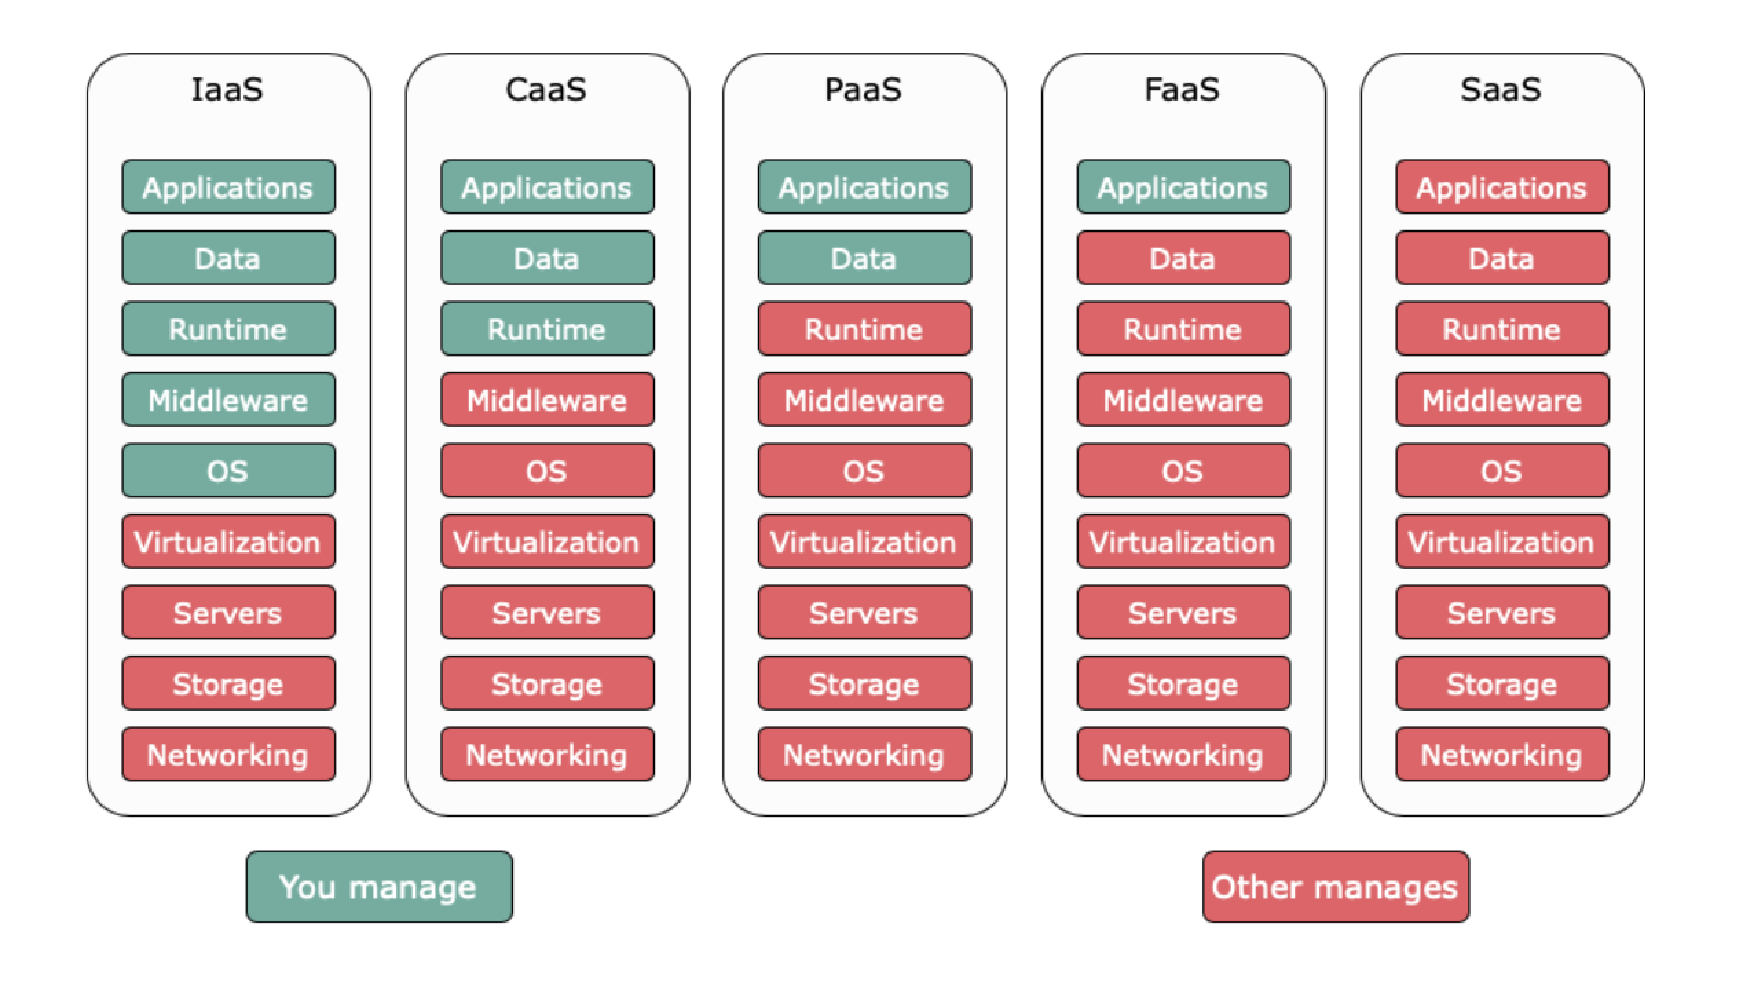
\includegraphics[width=\linewidth]{figures/IaaS_PaaS_FaaS.pdf}
    \caption{Servizi cloud computing}
    \label{fig:servizi-cloud-computing}
\end{figure}

\noindent
Il documento è organizzato nel seguente modo: il \cref{chap:frameworks} presenta i principali framework, specialmente Open Source; nel \cref{chap:setup-sperimentale} si individuano le metriche qualitative e quantitative, le quali verranno poi utilizzate per valutare i framework. Il \cref{chap:creazione-sistema-test} effettua una panoramica sulla configurazione dell'ambiente all'interno del quale verranno effettuati i test, oltre a presentare la loro configurazione e il loro obiettivo. All'interno del \cref{chap:risultati-sperimentali} vengono mostrati i grafici raffiguranti i risultati dei test e si effettua una breve analisi. Infine, nel \cref{chap:conclusioni} si effettua un riassunto degli aspetti più importanti individuati.

%Write your intro here.
%\sidenote{Add sidenotes in this way. They are named after the author of the thesis}

% You can use acronyms that your defined previously,
% such as \ac{IoT}.
% %
% If you use acronyms twice,
% they will be written in full only once
% (indeed, you can mention the \ac{IoT} now without it being fully explained).
% %
% In some cases, you may need a plural form of the acronym.
% %
% For instance,
% that you are discussing \acp{vm},
% you may need both \ac{vm} and \acp{vm}.

% \paragraph{Structure of the Thesis}

% \note{At the end, describe the structure of the paper}

% \chapter{State of the art}

% I suggest referencing stuff as follows: \cref{fig:random-image} or \Cref{fig:random-image}

% \begin{figure}
%     \centering
%     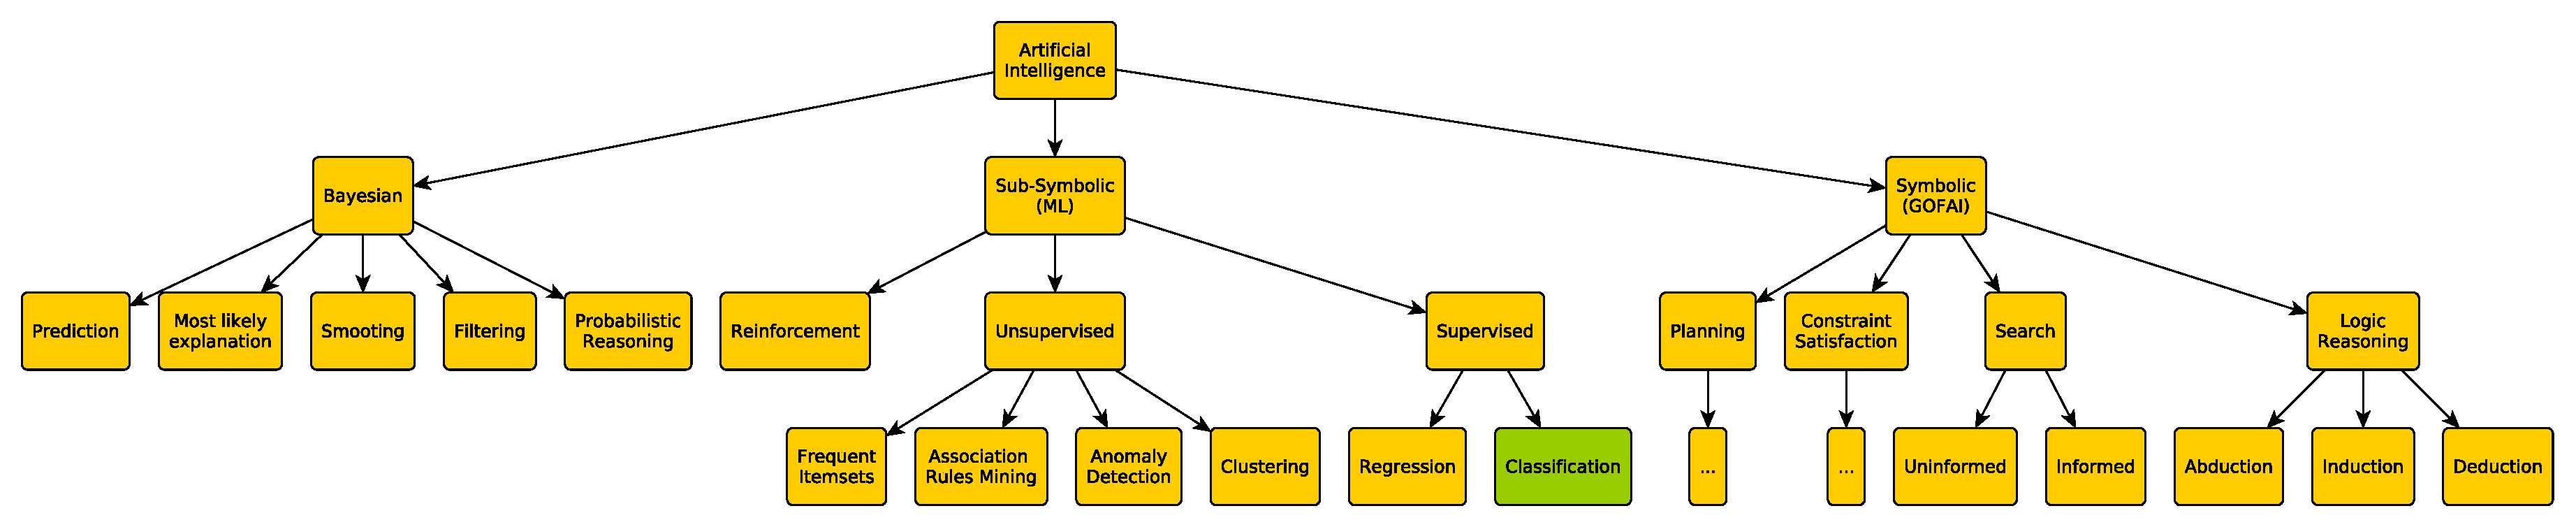
\includegraphics[width=.8\linewidth]{figures/random-image.pdf}
%     \caption{Some random image}
%     \label{fig:random-image}
% \end{figure}

% \section{Some cool topic}

%----------------------------------------------------------------------------------------
\chapter{Frameworks}
\label{chap:frameworks}
%----------------------------------------------------------------------------------------

Grazie al grande entusiasmo legato al serverless computing dal momento della sua introduzione, sono nati numerosi framework, ovvero strumenti che si occupano di eseguire le procedure operative del server, della rete, di bilanciamento del carico e di autoscaling~\cite{Palade2019}.
I framework si suddividono principalmente in due categorie:
\begin{enumerate}
    \item \textbf{Framework proprietari}: i quali sono gestiti da venditori esterni e quindi non mostrano le implementazioni delle funzionalità, non consentendo facilmente il passaggio ad un altro fornitore.
    
    \item \textbf{Framework Open Source}: sono stati introdotti per evitare il blocco verso un venditore (``vendor lock-in") e le restrizioni computazionali di una piattaforma cloud esterna.
\end{enumerate}

\section{Framework proprietari}

I framework proprietari sono gestiti da fornitori di terze parti, i quali offrono dei servizi a pagamento per poter usufruire della loro piattaforma. Inoltre, essendo gestiti a livello aziendale, non si è a conoscenza dell'implementazione e dell'effettiva realizzazione del servizio. Dato che sono prodotti commerciali non c'è alcun interesse da parte dell'azienda nel consentire un comodo passaggio dal loro framework ad un altro, causando il cosiddetto ``vendor lock-in".
Le principali alternative sono: AWS Lambda \footnote{\url{https://aws.amazon.com/it/lambda/}}, Azure Functions \footnote{\url{https://azure.microsoft.com/en-us/products/functions}}, IBM Cloud Code Engine \footnote{\url{https://cloud.ibm.com/codeengine/overview}} e Google Cloud Functions \footnote{\url{https://cloud.google.com/functions}}.

\subsection{AWS Lambda}

Si tratta di un servizio di elaborazione event-based, cioè esegue il codice in risposta ad eventi, gestendo automaticamente le risorse; questo consente di realizzare applicazioni serverless.
Lambda ha il compito di gestire ``load balancing", autoscaling, isolamento, etc; mentre consente il controllo della memoria, contrariamente alla percentuale di core della CPU e alla capacità della rete, le quali vengono assegnate proporzionalmente ad essa. In pratica, un'applicazione serverless che utilizza questo servizio lavora nel seguente modo: la sorgente di un evento provoca l'invocazione di una funzione (\textit{AWS Lambda functions}), la quale utilizza dei servizi esterni (es. database...).
Il componente principale utilizzato dal framework è l'\textbf{API gateway} che ha le seguenti caratteristiche:
\begin{itemize}
    \item gestisce autenticazione, autorizzazione e il routing delle applicazioni;
    
    \item crea un'\ac{api} di \textit{front-end} unificata;
    
    \item crea i \textit{WebSockets}, i quali suddividono la connessione in \textit{stateful connection} verso i client e \textit{stateless connection} nei confronti degli altri componenti.
\end{itemize}
I \textit{Lambda execution model}, che consistono nella modalità di invocazione delle funzioni e di gestione delle risposte, sono:
\begin{itemize}
    \item \textbf{Synchronous (push)}: la richiesta viene fatta dall'\textit{API gateway} e si aspetta la risposta della funzione.
    
    \item \textbf{Asynchronous (event)}: non si attende la risposta della funzione.
    
    \item \textbf{Poll-based}: avviene un costante controllo (``polling") degli stream di messaggi da parte di un servizio che richiama la funzione.
\end{itemize}

\section{Framework Open Source}

I framework Open Source non sono gestiti da una singola entità, ma da una serie di contributori che partecipano al miglioramento del codice, il quale è pubblico e consultabile da chiunque. Il vantaggio di questi framework è che nella maggior parte dei casi sono gratuiti, o quantomeno offrono un piano senza costi, con delle limitazioni nelle risorse concesse. Principalmente sono stati introdotti per consentire il facile passaggio tra varie soluzioni, aggirando quindi il ``vendor lock-in" e tutte le limitazioni di una piattaforma proprietaria~\cite{Yussupov2021}. Questi sono formati da vari componenti, che spesso sono altri prodotti Open Source, i quali vengono assemblati per fornire un'infrastruttura completa.
I framework Open Source di serverless computing sono numerosi, ma i principali sono:
\begin{enumerate}
    \item \textbf{Kubeless}\footnote{\url{https://github.com/vmware-archive/kubeless/tree/maste}}
    
    \item \textbf{Apache OpenWhisk}\footnote{\url{https://openwhisk.apache.org/}}
    
    \item \textbf{OpenFaaS}\footnote{\url{https://www.openfaas.com/}}
    
    \item \textbf{Knative}\footnote{\url{https://knative.dev/}}
\end{enumerate}

\subsection{Kubeless}

Si tratta di un framework serverless nativo di Kubernetes \footnote{\url{https://kubernetes.io/}}.
\\
Le sue primitive sono:
\begin{itemize}
    \item \textbf{Functions}: consistono nel codice che deve essere eseguito.
    
    \item \textbf{Triggers}: sono le sorgenti degli eventi e possono essere associati a una funzione o ad un gruppo di funzioni.
    
    \item \textbf{Runtime}: sono il linguaggio e l'ambiente dove verrà eseguita la funzione.
\end{itemize}
Il componente principale è:
\begin{itemize}
    \item \textbf{CRD controller}: è colui il quale osserva continuamente i \textit{Function objects} in cerca di cambiamenti ed effettua di conseguenza le azioni necessarie (es. creazione o eliminazione di un \textit{Function object}).
\end{itemize}

\subsection{Apache OpenWhisk}

Consiste in un servizio serverless di programmazione event-driven, il cui modello è rappresentato nella \Cref{fig:modello-apache-openwhisk}.
\\
Le sue primitive sono:
\begin{itemize}
    \item \textbf{Actions}: sono \textit{stateless function} che eseguono codice. È possibile comporne molteplici per creare una pipeline detta \textit{sequence}.
    
    \item \textbf{Triggers}: consistono in classi di eventi che possono avere origine da varie fonti.
    
    \item \textbf{Rules}: associano un \textit{Trigger} ad una \textit{Action}.
\end{itemize}

\begin{figure}[ht]
    \centering
    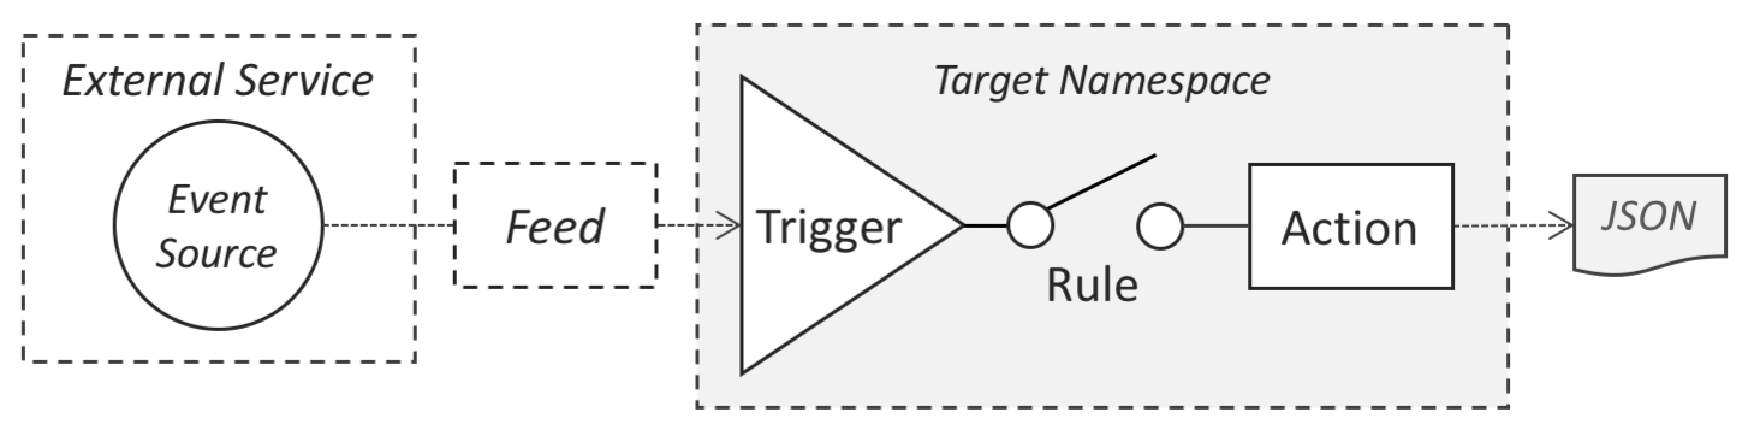
\includegraphics[width=\linewidth]{figures/Programming_model_OpenWhisk.pdf}
    \caption{Modello Apache OpenWhisk}
    \label{fig:modello-apache-openwhisk}
\end{figure}
\noindent
I componenti principali che lo compongono, come si può osservare nella \Cref{fig:architettura-apache-openWhisk}, sono:
\begin{itemize}
    \item \textbf{Nginx webserver}: agisce da server proxy ed è il primo \textit{entrypoint}.
    
    \item \textbf{Controller}: si occupa di autenticazione, autorizzazione e instradamento di ogni richiesta.
    In pratica traduce la richiesta ricevuta da \textit{Nginx} nell'invocazione di un'azione. Inoltre, contiene un \textit{Load Balancer} che si occupa di scegliere a quale \textit{Invoker} affidare la richiesta in base al carico.
    
    \item \textbf{Apache Kafka}: gestisce le connessioni tra il \textit{Controller} e l'\textit{Invoker}, infatti si tratta di un sistema di messaggistica \textit{publish-subscribe} distribuito e ad alta portata.
    
    \item \textbf{Invoker}: si occupa di copiare il codice da \textit{CouchDB} ed iniettarlo in un container Docker\footnote{\url{https://www.docker.com/}}; questo viene sfruttato per consentire l'esecuzione delle azioni in modo sicuro ed isolato.
    
    \item \textbf{CouchDB}: consiste in un database, all'interno del quale vengono memorizzati anche i risultati delle invocazioni. Si occupa di fornire al \textit{Controller} l'azione richiesta ed inoltre mantiene tutte le attivazioni collezionate per id.
\end{itemize}

\begin{figure}[ht]
    \centering
    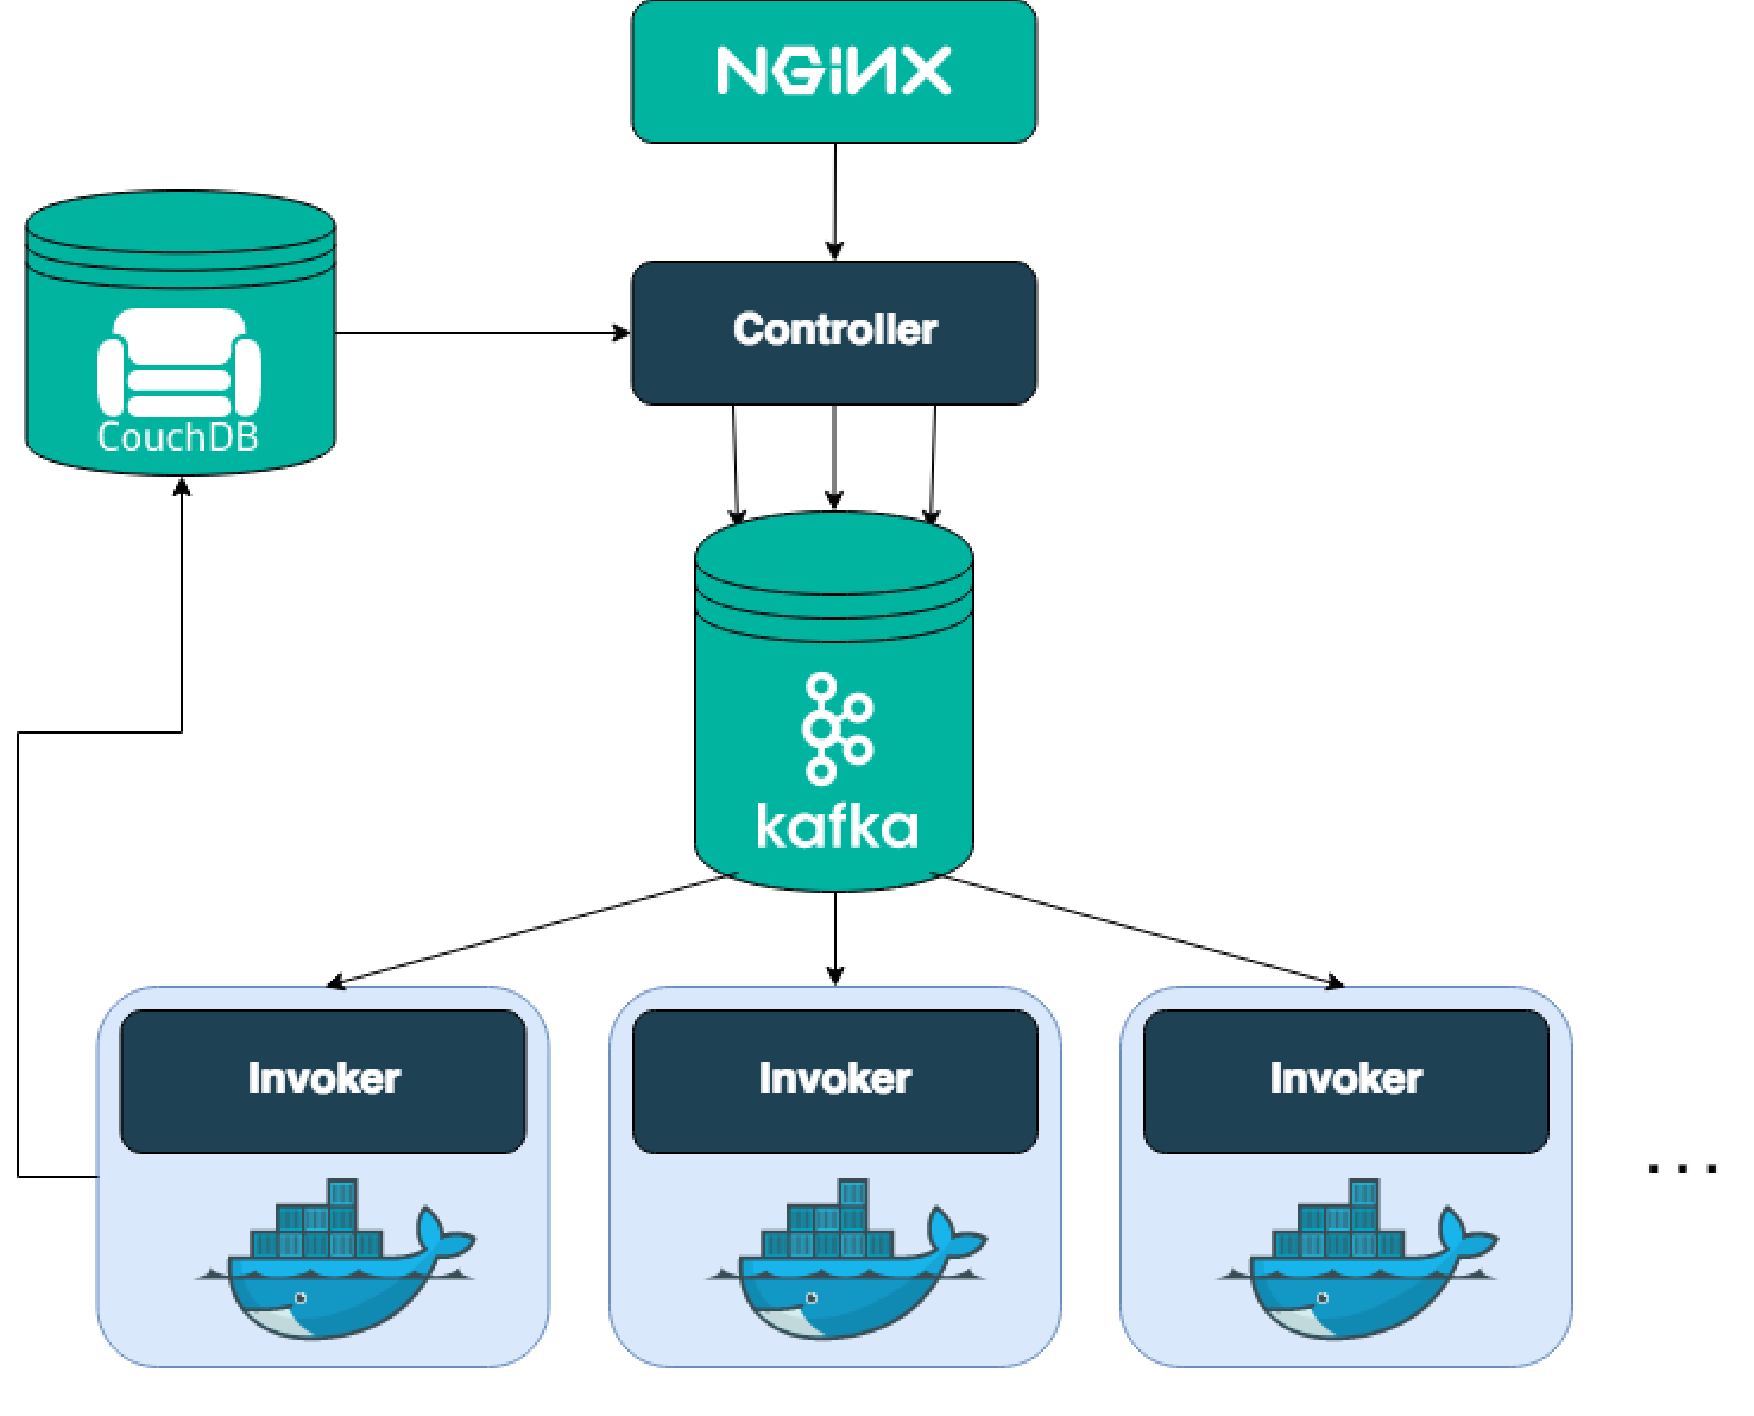
\includegraphics[width=\linewidth]{figures/OpenWhisk_schema.pdf}
    \caption{Architettura Apache OpenWhisk}
    \label{fig:architettura-apache-openWhisk}
\end{figure}

\subsubsection{Creazione e invocazione di una Action}

È innanzitutto necessario scegliere un linguaggio e successivamente attenersi ai seguenti passi:
\begin{enumerate}
    \item creazione di un file con il codice che l'azione deve eseguire (es. in Java creazione di un file \texttt{MyAction.java} contenente la classe \texttt{MyAction});
    
    \item \textit{[opzionale]} svolgimento dei passaggi specifici del linguaggio scelto (es. in Java è richiesta la compilazione del file e la creazione del \texttt{jar});
    
    \item creazione dell'azione con il comando:\begin{lstlisting}
wsk action create myAction myAction.jar --main MyAction\end{lstlisting}
    dove con il flag \texttt{--main} si specifica l'entrypoint;
    
    \item invocazione dell'azione ed ottenimento del risultato grazie al flag \texttt{--result}, mediante il comando che segue:\begin{lstlisting}
wsk action invoke myAction --result\end{lstlisting}
    
    \item \textit{[opzionale]} il \texttt{deploy} con \texttt{wskdeploy} è realizzabile tramite i passi che seguono:
        \begin{itemize}
            \item creazione del file \texttt{manifest.yaml}, eg: \cref{lst:manifest}; 
            
            \lstinputlisting[float,label={lst:manifest},caption={\texttt{manifest.yaml}}]{listings/manifest.yaml}
            
            \item \texttt{deploy} sfruttando il file creato in precedenza:\begin{lstlisting}
wskdeploy -m manifest.yaml\end{lstlisting}
        \end{itemize}
\end{enumerate}
Questi passaggi potrebbero subire leggere variazioni in base al linguaggio scelto.
\\ \\
L'invocazione di una \textit{Action} può essere effettuata, in alternativa al comando \texttt{wsk action invoke myAction}, citato in precedenza, inviando richieste \ac{http} (per esempio tramite il comando \texttt{curl}) all'indirizzo fornito a seguito del \texttt{deploy} della funzione, che corrisponde all'\textit{API HOST}, il quale è configurabile a piacimento.

\subsubsection{Package}

I \textbf{packages} servono per impacchettare un insieme di azioni correlate, permettendo anche la loro condivisione. Ci sono vari \textit{package} pubblici messi a disposizione dal framework all'interno del namespace \texttt{/whisk.system}, i quali offrono diverse funzionalità e accesso a servizi esterni, come \textit{GitHub}\footnote{\url{https://github.com/}}, \textit{Slack}\footnote{\url{https://slack.com/}}, etc.
\newline
Il sottocomando per ottenere informazioni sui \textit{package} è: \begin{lstlisting}
wsk package\end{lstlisting}

\noindent
Ci sono due modalità di invocazione di un'azione da un \textit{package}:
\begin{enumerate}
    \item direttamente dal suo interno, nella seguente modalità:
        \begin{itemize}
            \item recapito della descrizione dell'azione: \begin{lstlisting}
wsk action get --summary /whisk.system/samples/greeting\end{lstlisting}
            \item invocazione dell'azione con parametri opzionali: \begin{lstlisting}
wsk action invoke --result /whisk.system/samples/greeting --param name Bernie --param place Vermont\end{lstlisting}
        \end{itemize}
    
    \item creazione di un \textit{package binding}, con successiva invocazione dell'azione nel ``binding":
    \begin{lstlisting}
wsk package bind /whisk.system/samples valhallaSamples
wsk action invoke --result valhallaSamples/greeting --param name Odin\end{lstlisting}
\end{enumerate}

\subsubsection{Trigger}

Servono ad automatizzare \textit{Actions} in risposta ad eventi provenienti da \textit{Event Sources}.

\paragraph{\underline{Creazione ed esecuzione Trigger}} ~
\begin{itemize}
    \item creazione di un \textit{Trigger}:
    \begin{lstlisting}
wsk trigger create myTrigger\end{lstlisting}
    
    \item esecuzione del \textit{Trigger} specificando il nome e facoltativamente alcuni parametri:
    \begin{lstlisting}
wsk trigger fire myTrigger --param <key> <value>\end{lstlisting}
\end{itemize}

\paragraph{\underline{Associazione tra Trigger e Action tramite Rule}} ~\\
Si crea una \textit{Rule} che associa un \textit{Trigger} ad una \textit{Action}, entrambi già esistenti:
\begin{lstlisting}
wsk rule create myRule myTrigger myAction\end{lstlisting}

\paragraph{\underline{Invocazione Action mediante Trigger}} ~
\begin{lstlisting}
wsk trigger fire myTrigger --param <key> <value> --param <key> <value>\end{lstlisting}

\subsubsection{Flow del processo}

Si mostra una sequenza ordinata di fasi che descrive il processo esecutivo generale, ognuna caratterizzata da un componente dell'architettura:
\begin{enumerate}
    \item \textbf{Nginx} \\
    Si tratta del primo entrypoint del sistema.
    Il comando inviato tramite la \ac{cli} \texttt{wsk} è essenzialmente una richiesta \ac{http} e si traduce in:
    \\
    \texttt{POST /api/v1/namespaces/\$userNamespace/actions/myAction \\Host: \$openwhiskEndpoint}
    
    \item \textbf{Controller} \\
    Consiste in un'implementazione basata su Scala\footnote{\url{https://www.scala-lang.org/}} della \ac{rest} \ac{api}, che funge da interfaccia per tutto ciò che l'utente può fare. Il \textit{Controller} chiarisce ciò che vuole fare l'utente, basandosi sul metodo \ac{http} specificato nella richiesta (es. la richiesta, che sfrutta il metodo POST, di un'azione esistente viene tradotta nell'invocazione di una \textit{Action}).
    
    \item \textbf{CouchDB: autenticazione e autorizzazione} \\
    Il \textit{Controller} effettua alcune verifiche di autenticazione e autorizzazione tramite il controllo delle credenziali presenti nel database \textit{CouchDB}.
    
    \item \textbf{CouchDB: ottenere l'azione} \\
    Il \textit{Controller} carica l'\textit{Action} dal database \textit{Whisks} in \textit{CouchDB}. Il record dell'azione contiene il codice da eseguire, completato con i parametri passati nella richiesta; inoltre possiede le restrizioni delle risorse imposte per l'esecuzione.
    
    \item \textbf{Load Balancer} \\
    Si tratta di una parte del \textit{Controller} che ha una visione globale degli esecutori (\textit{Invokers}) disponibili, controllando continuamente il loro stato di salute (``health status"). Il \textit{Load Balancer} sceglie in base al carico un \textit{Invoker} per l'azione richiesta.
    
    \item \textbf{Kafka} \\
    Si tratta di un sistema di messaggistica \textit{publish-subscribe}, distribuito e ad elevato rendimento.
    Si occupa della gestione dei possibili errori, come i seguenti:
    \begin{itemize}
        \item il sistema va in ``crash", perdendo l'invocazione;
        \item il sistema viene sovraccaricato e quindi l'invocazione deve aspettare che ne finiscano altre prima.
    \end{itemize}
    Si occupa inoltre, di rendere persistente e ``bufferizzata" la comunicazione tra \textit{Controller} e \textit{Invoker}:
    \begin{enumerate}
        \item il \textit{Controller} pubblica un messaggio a \textit{Kafka} che contiene l'azione e i parametri;
        \item il messaggio viene indirizzato all'\textit{Invoker} scelto;
        \item dopo che \textit{Kafka} ha confermato la ricezione del messaggio, la richiesta viene risposta con un \textbf{ActivationId} (usato in seguito per accedere ai risultati dell'invocazione).
    \end{enumerate}
    
    \item \textbf{Invoker} \\
    Il suo compito è quello di invocare un'azione. La sua implementazione è in Scala e per l'esecuzione isolata e sicura di \textit{Actions} sfrutta Docker, il quale viene usato per creare un container per ogni azione invocata, in modo veloce, sicuro e isolato.
    Funzionamento:
    \begin{enumerate}
        \item creazione di un container Docker per ogni invocazione;
        \item il codice dell'azione viene iniettato al suo interno;
        \item il codice viene eseguito utilizzando anche i parametri;
        \item una volta ottenuto il risultato, il container viene distrutto.
    \end{enumerate}
    Viene anche effettuata un'ottimizzazione delle performance per ridurre l'``overhead" e diminuire i tempi di risposta.
    
    \item \textbf{CouchDB: archiviare i risultati} \\
    Il risultato ottenuto dall'\textit{Invoker} viene archiviato nel database \textit{activations} (all'interno di \textit{CouchDB}) per \texttt{ActivationId}.
    Il risultato consiste in un oggetto \texttt{JSON} ottenuto dall'azione, unito al log scritto da Docker, eg: \cref{lst:log}.

    \lstinputlisting[float,label={lst:log},caption={\texttt{log.json}}]{listings/log.json}

    A questo punto si può ricominciare dal passo 1 sfruttando nuovamente la \ac{rest} \ac{api} per ottenere l'attivazione e quindi il risultato dell'azione:
    \begin{lstlisting}
wsk activation result activationId\end{lstlisting}
\end{enumerate}

\subsubsection{API gateway}

L'\textit{\ac{api} gateway} agisce da proxy per \textbf{Web Actions} e fornisce loro funzionalità aggiuntive, come metodo di routing \ac{http}, limitazioni di rate, etc.

\paragraph{\underline{Creazione Web Action (uso di JavaScript)}}
\begin{enumerate}
    \item Creazione di un file JavaScript (es. \texttt{hello.js} \cref{lst:hello-js}).

    \lstinputlisting[float,language=JavaScript,label={lst:hello-js},caption={\texttt{hello.js}}]{listings/hello.js}
    
    \item Creazione di una \textit{Web Action} dalla seguente funzione Javascript:
    \begin{lstlisting}
wsk action create hello hello.js --web true\end{lstlisting}

    \item Creazione di un'\ac{api} con percorso base \texttt{/hello}, percorso \texttt{/world} e metodo \texttt{get} con tipo di risposta \texttt{JSON}:
    \begin{lstlisting}
wsk api create /hello /world get hello --response-type json\end{lstlisting}

    In questo modo è stato generato un nuovo \ac{url} che espone l'azione \texttt{hello} tramite metodo \ac{http} GET.
    
    \item Si può verificare inviando una richiesta \ac{http} all'\ac{url} generato in precedenza, per esempio sfruttando il comando \texttt{curl}:
    \begin{lstlisting}
curl https://${APIHOST}:9001/api/${GENERATED_API_ID}/hello/world?name=OpenWhisk\end{lstlisting}
\end{enumerate}

\subsubsection{Opzioni di deployment}

L'opzione di deployment consigliata è Kubernetes, perché è supportata dalla maggior parte delle piattaforme ed offre molte possibilità sia per lo sviluppo locale che per produzione su larga scala. Ad ogni modo si mostrano tutte le possibilità di deployment che OpenWhisk mette a disposizione.

\paragraph{\underline{Kubernetes}} ~\\
OpenWhisk può essere dispiegato usando gli \textit{Helm\footnote{\url{https://helm.sh/}} Charts} su qualsiasi Kubernetes fornito localmente o da un ``cloud provider" pubblico.

\paragraph{\underline{Standalone OpenWhisk Stack}} ~\\
Si tratta di uno stack completo che viene eseguito come un processo Java. Le \textbf{serverless functions} vengono eseguite dentro container Docker; quindi è necessario aver installato localmente Docker, Java e Node.js\footnote{\url{https://nodejs.org/}}.
I passaggi richiesti sono:
\begin{itemize}
    \item clonazione del repository e creazione dello stack:
    \begin{lstlisting}
$ git clone https://github.com/apache/openwhisk.git
$ cd openwhisk
$ ./gradlew core:standalone:bootRun\end{lstlisting}

    \item Una volta che lo stack è stato creato si aprirà il browser in un \textit{functions playground}, solitamente all'indirizzo \texttt{http://localhost:3232}, che permette la creazione e l'esecuzione delle funzioni direttamente nel browser.
\end{itemize}

\paragraph{\underline{Docker Compose}} ~\\
Docker Compose\footnote{\url{https://docs.docker.com/compose/}} è la scelta giusta nel caso in cui si voglia utilizzare direttamente Docker. 
\begin{lstlisting}
$ git clone https://github.com/apache/openwhisk-devtools.git
$ cd openwhisk-devtools/docker-compose
$ make quick-start\end{lstlisting}

\paragraph{\underline{Ansible}} ~\\
Il deployment sfruttando Ansible\footnote{\url{https://www.ansible.com/}} consiste in un approccio più imperativo, basato su script. Gli \textbf{OpenWhisk playbooks} sono strutturati in modo da consentire il ``cleaning", ``deploying" o ``re-deploying" di un singolo componente come dell'intero stack.

\paragraph{\underline{Vagrant}} ~\\
Vagrant\footnote{\url{https://www.vagrantup.com/}} per essere utilizzato richiede l'installazione di VirtualBox\footnote{\url{https://www.virtualbox.org/}}, per gestire la virtualizzazione dell'hardware.

\subsection{OpenFaaS}

Questo framework si appoggia su Kubernetes e Docker, infatti ogni funzione è impacchettata in un container Docker isolato dal resto dell'architettura, la quale viene mostrata nella \Cref{fig:architettura-openfaas}. Ogni container inoltre contiene un \textbf{watchdog}, ovvero una guardia.
\\
Le sue primitive sono:
\begin{itemize}
    \item \textbf{Functions}: lo sviluppatore ha il compito di fornire la funzione ed un \texttt{Handler}.
\end{itemize}

\noindent
I principali componenti che lo formano sono:
\begin{itemize}
    \item \textbf{API gateway}: fornisce accesso alle funzioni, colleziona le metriche e fornisce autoscaling, interagendo con l'\textit{orchestration engine} (es. Kubernetes).
    \item \textbf{AlertManager\footnote{\url{https://github.com/prometheus/alertmanager}} o Kubernetes \ac{hpa}\footnote{\url{https://kubernetes.io/docs/tasks/run-application/horizontal-pod-autoscale/}}}: nel primo caso è combinato con \textbf{Prometheus}\footnote{\url{https://prometheus.io/}}, mentre nel secondo si tratta dell'\ac{hpa} di Kubernetes. 
\end{itemize}

\begin{figure}[ht]
    \centering
    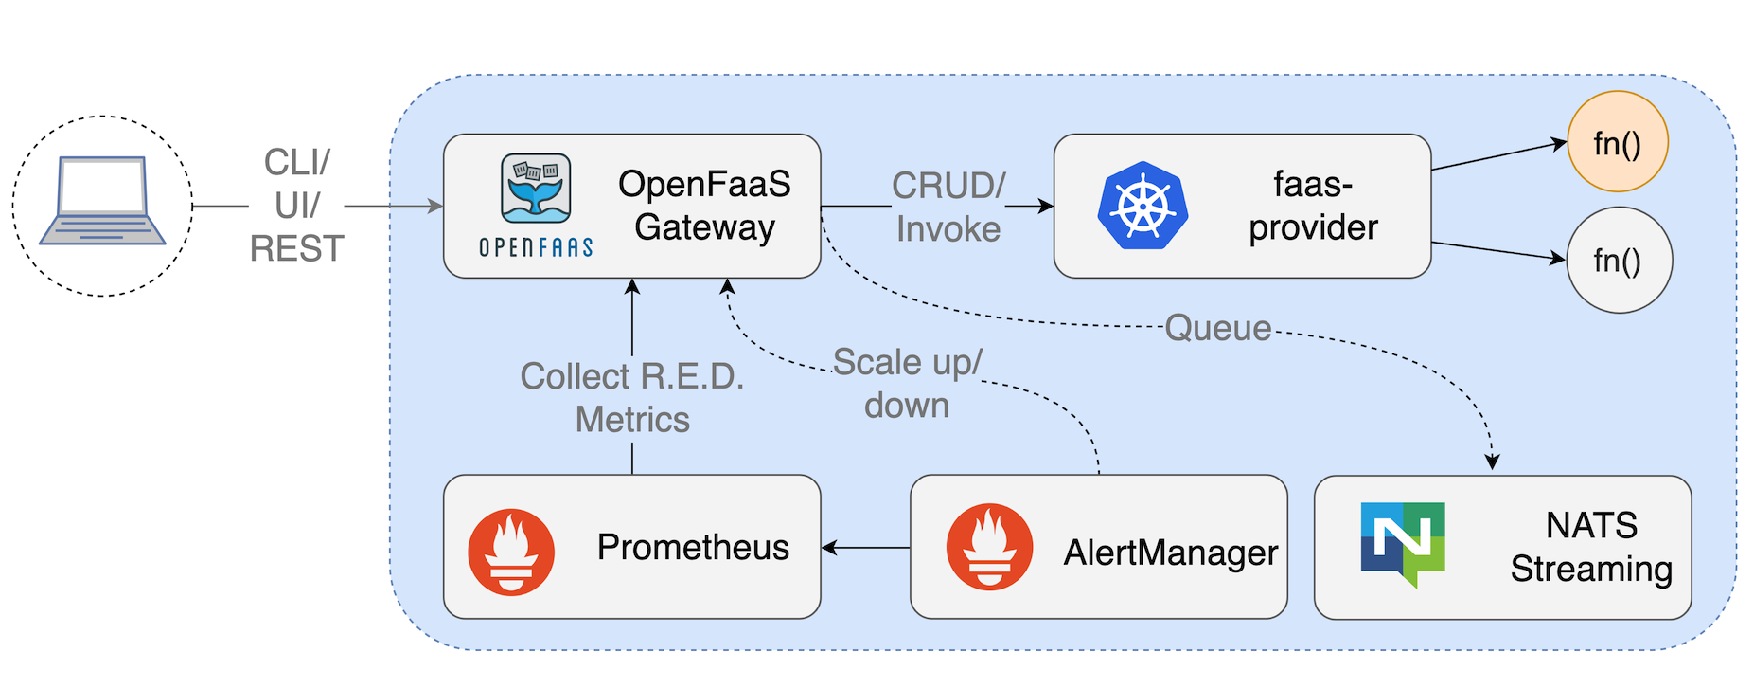
\includegraphics[width=\linewidth]{figures/OpenFaaS_architecture.pdf}
    \caption{Architettura OpenFaaS}
    \label{fig:architettura-openfaas}
\end{figure}

\subsubsection{Workflow}

\begin{itemize}
    \item Tutti i servizi e le funzioni prendono una route esposta di default, ma possono essere usati domini personalizzati per ogni \textit{endpoint};
    
    \item  cambiando l'\ac{url} legato ad una funzione da \texttt{/function/NAME} a \\
    \texttt{/async-function/NAME}, un'invocazione può essere eseguita in una coda usando il componente \textbf{NATS Streaming} (mostrato nella \Cref{fig:architettura-openfaas});
    
    \item \textbf{faas-netes} è l'\textit{orchestration provider} più popolare. I provider sono costruiti con il \textit{faas-provider \ac{sdk}}.
\end{itemize}

\subsubsection{Deployment}

In questa sezione si fa riferimento alla versione \textbf{OpenFaaS CE}.
\begin{enumerate}
    \item Creazione di un cluster Kubernetes, il quale deve avere sempre completo accesso ad Internet.
    \\
    Alcune opzioni per cluster locali sono:
    \begin{itemize}
        \item KinD\footnote{\url{https://kind.sigs.k8s.io/}}: effettua l'``upstream" di Kubernetes in un container con Docker;
        
        \item K3s\footnote{\url{https://k3s.io/}}: distribuzione di Kubernetes leggera, ideale per lo sviluppo, \ac{IoT} e dispositivi \textit{at the edge};
        
        \item K3d\footnote{\url{https://k3d.io/}}: come K3s, ma in un container Docker; infatti consiste in un \textit{lightweight wrapper} per eseguire K3s;
        
        \item minikube\footnote{\url{https://minikube.sigs.k8s.io/}}: creazione di cluster Kubernetes nella macchina locale tramite una \ac{vm} separata.
    \end{itemize}

    Opzioni per cluster remoti:
    \begin{itemize}
        \item K3sup\footnote{\url{https://github.com/alexellis/k3sup}}: costruzione di cluster a nodo singolo o multiplo usando ``cloud \acp{vm}".
    \end{itemize}
    
    \item Installazione della \ac{cli} \textbf{faas-cli} per la gestione ed il \texttt{deploy} delle funzioni;
    
    \item installazione di \textbf{OpenFaaS CE} tramite Arkade\footnote{\url{https://github.com/alexellis/arkade}} (consigliato) oppure Helm;
    
    \item ogni volta che una funzione è dispiegata o scalata verso l'alto, Kubernetes farà il \texttt{pull} di una copia potenzialmente aggiornata dell'immagine dal registry, a meno che la relativa opzione non sia stata configurata a \texttt{Never}, in quel caso funzioneranno solo le immagini locali.
\end{enumerate}

\subsubsection{Creazione e gestione funzione}

\paragraph{\underline{Creazione funzione}} ~\\
Il framework mette a disposizione un archivio da cui è possibile scaricare vari template:
\begin{lstlisting}
$ faas-cli template store list
$ faas-cli template store pull <template-name>\end{lstlisting}
Una volta fatto questo si può creare una funzione utilizzando il template scaricato:
\begin{lstlisting}
faas-cli new --lang <template-name> <function-name>\end{lstlisting}
Il codice della funzione può essere modificato all'interno del file \texttt{Handler}.

\paragraph{\underline{Costruzione funzione}} ~\\
Le funzioni sono costruite come immagini di container compatibili con il formato \ac{oci}, che di solito contengono il \textit{watchdog} come proxy. Quando si esegue il seguente comando usando un template dal negozio, l'immagine del container sarà costruita nella libreria locale:
\begin{lstlisting}
faas-cli build\end{lstlisting}
I template tendono ad astrarre il \textit{Dockerfile} e l'\textit{entrypoint \ac{http} server}, permettendo di concentrarsi su un \textbf{\ac{http}/functions handler}.

\paragraph{\underline{Risultato della creazione di una funzione}} ~\\
Ogni funzione che ha subito \texttt{deploy}, creerà un oggetto separato \textit{Kubernetes Deployment}; esso ha un valore \textbf{replicas}, il quale corrisponde al numero di \textit{Pods} creati nel cluster. Viene anche creato un oggetto \textit{Kubernetes Service}, il quale è usato per accedere all'endpoint \ac{http} della funzione sulla porta 80 dentro il cluster.
Di norma le funzioni hanno un numero minimo di repliche uguale a uno, in modo da prevenire la \textbf{cold start}, infatti in questo modo non deve essere creato ogni volta un \textit{Pod} per gestire una richiesta. Per \textit{cold start} si intende il processo che richiede l'avvio di una nuova istanza di una funzione, ma nel caso di un framework \ac{FaaS} questo potrebbe anche comportare la necessità della creazione e configurazione di un nuovo container, con il conseguente \texttt{deploy} della funzione; dunque nel suddetto contesto i tempi di gestione di una richiesta aumenterebbero notevolmente~\cite{216063}.
Per quanto riguarda invece il limite delle invocazioni che possono essere effettuate nei confronti di una funzione, è possibile impostarlo tramite la variabile d'ambiente \texttt{max\_inflight: N}, altrimenti di default non è presente alcun limite.

\paragraph{\underline{Deploy funzione}} ~\\
Per eseguire il \texttt{deploy} di una funzione, si può utilizzare il comando \texttt{up}, oppure eseguire i singoli comandi che esso racchiude, singolarmente:
\begin{itemize}
    \item in caso di comando singolo: \begin{lstlisting}
faas-cli up -f <function-name>.yml\end{lstlisting}
    \item In caso di separazione dei comandi: \begin{lstlisting}
$ faas-cli build -f <function-name>.yml
$ faas-cli push -f <function-name>.yml
$ faas-cli deploy -f <function-name>.yml\end{lstlisting}
\end{itemize}

\subsubsection{Invocazioni}

Le funzioni possono essere invocate tramite richieste \ac{http} all'\textbf{OpenFaaS gateway} oppure sfruttando il comando:\begin{lstlisting}
faas-cli invoke\end{lstlisting}
\noindent
Ogni funzione è dispiegata sotto forma di \textit{Kubernetes Deployment and Service}, con un determinato numero di repliche; quindi può scalare verso l'alto e il basso, oltre a gestire più richieste concorrenti.

\paragraph{\underline{Invocazioni sincrone e asincrone}} ~\\
\begin{enumerate}
    \item \underline{Invocazioni sincrone:} si può invocare il \textit{gateway} con una richiesta \ac{http} all'indirizzo \texttt{http://<GATEWAY\_IP>:<PORT>/function/NAME}, dove \texttt{NAME} è il nome della funzione, \texttt{GATEWAY\_IP} e \texttt{PORT} sono l'indirizzo e la porta dell'\textit{API gateway}. È possibile avere anche uno strato intermedio, come un \textit{reverse proxy}. La connessione tra il chiamante e la funzione rimane sempre attiva, finché l'invocazione non è completata o scaduta.
    \item \underline{Invocazioni asincrone:} le richieste \ac{http} sono messe in una coda del \textbf{NATS Streaming}, seguite da un \textit{header} \texttt{accepted} e un \textit{call-id} ritornati al chiamante. Successivamente un \textbf{queue-worker} separato, prende il messaggio dalla coda ed invoca la funzione in modo sincrono. Non c'è mai una connessione diretta tra chiamante e funzione.
\end{enumerate}

\subsubsection{Events}
Per ogni \textit{event trigger} un \textbf{long-running daemon} è sottoscritto ad un topic o ad una coda, poi quando riceve dei messaggi, cerca le funzioni pertinenti e le invoca in maniera sincrona o asincrona.

\subsubsection{Autenticazione}

La \textbf{\ac{rest} \ac{api}} è usata per gestire le funzioni ed implementa di default le tecniche di autenticazione basiche; è possibile inoltre abilitare la crittografia tramite \ac{tls} e un \textit{reverse proxy}.
Si possono gestire le funzioni con la \textit{Function \ac{crd}}, che è osservata da un operatore, il quale può creare risorse in Kubernetes, oltrepassando la \ac{rest} \ac{api} del \textit{gateway}; quest'ultima viene utilizzata comunque per le invocazioni. Per quanto riguarda le funzioni spetta invece allo sviluppatore fornire un meccanismo di autenticazione.

\subsubsection{Gateway}

Ogni funzione è costruita in un'immagine Docker immutabile, prima di essere dispiegata con \textit{faas-cli}, \ac{ui} o \ac{rest} \ac{api}.
Quando si effettua il \texttt{deploy} di una funzione si creano da uno a molti \textit{Pods/containers}, in base al numero minimo e massimo specificati nei parametri di scalabilità.
Nella \Cref{fig:openfaas-gateway} si notano i componenti di OpenFaaS, tra cui il \textit{gateway}, all'interno di un diagramma concettuale della piattaforma.

\begin{figure}[ht]
    \centering
    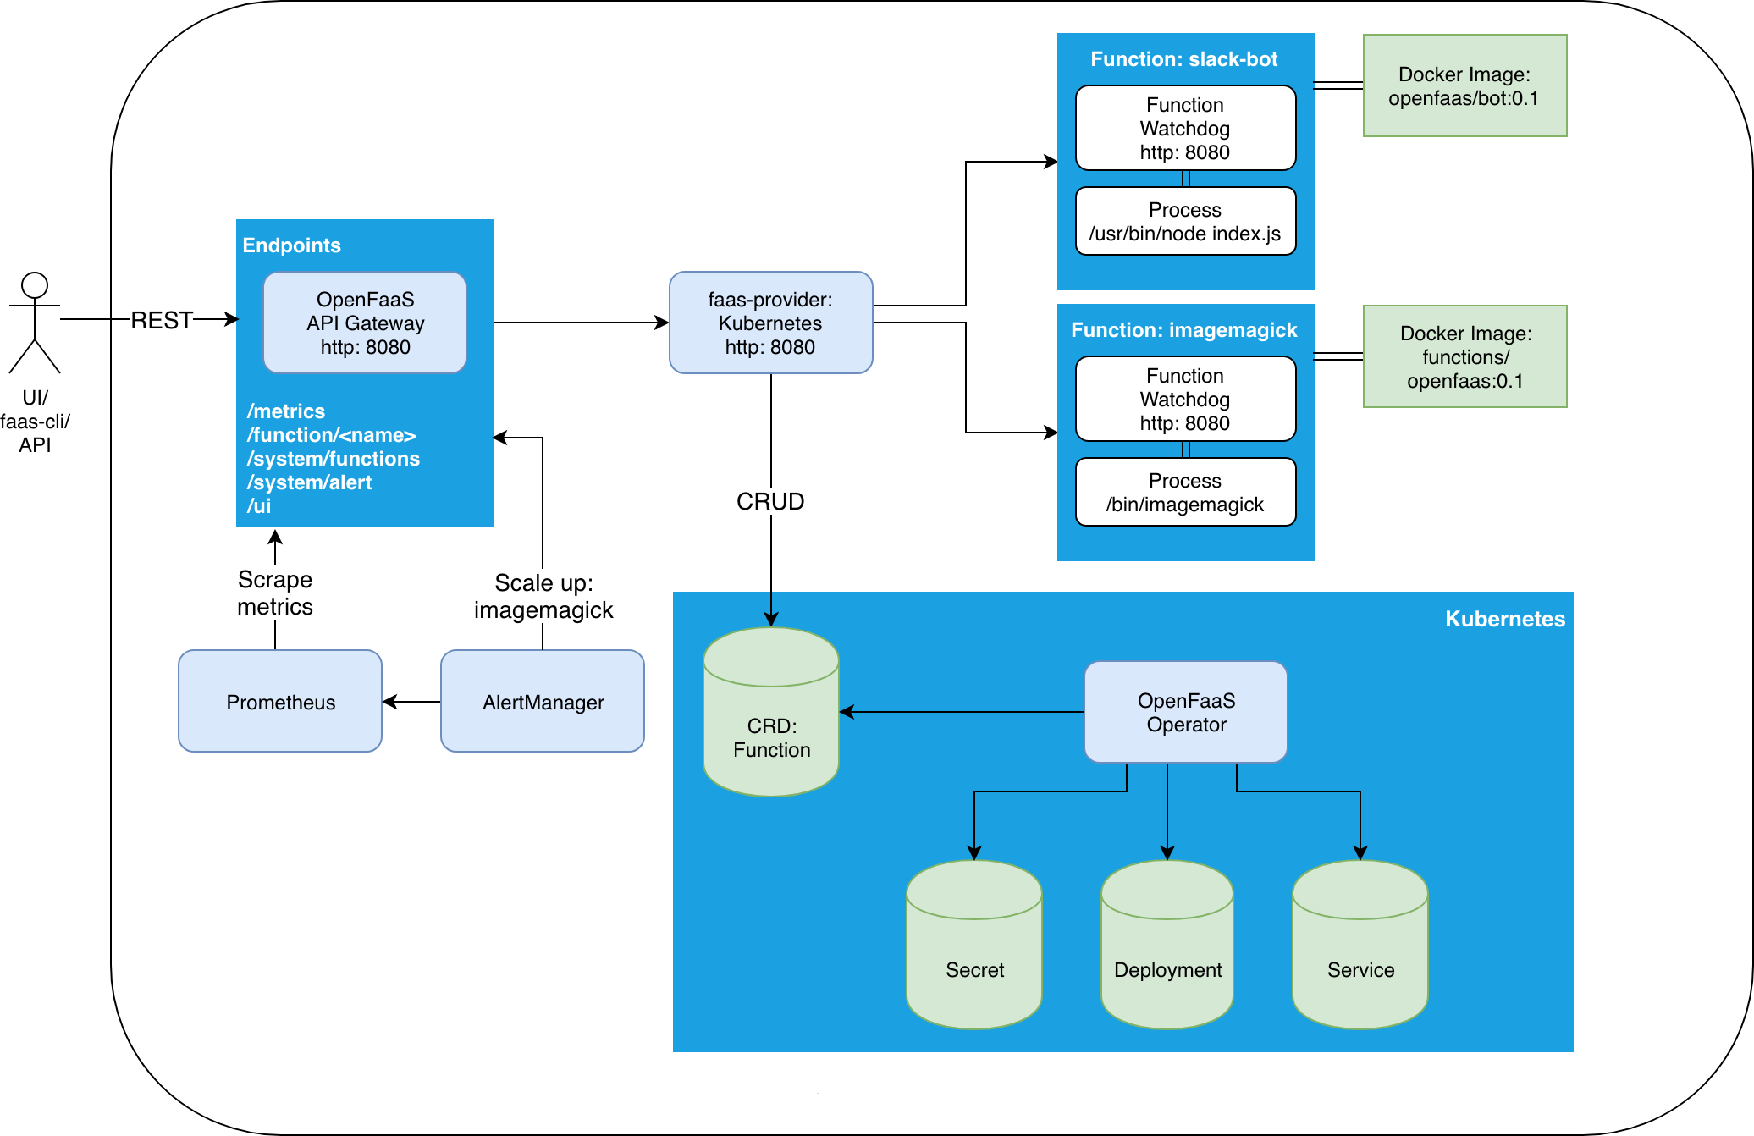
\includegraphics[width=\linewidth]{figures/OpenFaaS_gateway.pdf}
    \caption{OpenFaaS Gateway}
    \label{fig:openfaas-gateway}
\end{figure}

\subsubsection{Watchdog}

Si tratta del responsabile dell'avvio e del monitoraggio delle funzioni. Ogni file binario con un \textbf{watchdog} può diventare una funzione; questo diventa un \textit{init process} con un \textit{embedded \ac{http} server} scritto in Golang\footnote{\url{https://go.dev/}}, il quale può supportare richieste concorrenti, timeout e controlli dello stato.

\paragraph{\underline{Watchdog classico}} ~\\
Fornisce un'interfaccia tra l'esterno e la funzione; inoltre avvia un processo per ogni richiesta e usa \texttt{stdio} per la comunicazione. Ogni funzione deve incorporare questo binario e usarlo come entrypoint, cioè come \textit{init process}. Una volta che il processo è stato ``forked", il \textit{watchdog} passa alla richiesta \ac{http} via \texttt{stdin} e legge una risposta via \texttt{stdout}; quindi non è necessario che il processo sappia qualcosa del web o di \ac{http}.

\paragraph{\underline{of-watchdog}} ~\\
Si tratta di un progetto complementare a quello classico. Fornisce un'alternativa a \texttt{stdio} per la comunicazione tra il watchdog e la funzione. La principale differenza è che consente di mantenere il processo della funzione ``caldo" tra le invocazioni. Questo watchdog infatti abilita una modalità \texttt{http}, dove lo stesso processo può essere riusato ripetutamente per compensare la latenza del \textit{forking}; inoltre abilita il riutilizzo della memoria e la risposta rapida alle richieste. Il componente implementa un server \ac{http} in ascolto sulla porta 8080 e agisce da \textit{reverse proxy} per eseguire funzioni e microservizi.
\\
Ci sono varie modalità di interazione con il microservizio o la funzione:
\begin{itemize}
    \item \texttt{\ac{http}}: è l'opzione di default e quella più efficiente se il target ha un server \ac{http};
    
    \item \texttt{serializing}: quando non c'è l'implementazione di un server \ac{http}, allora \texttt{stdio} è letto dalla memoria e poi inviato in un processo ``forked";
    
    \item \texttt{streaming}: analoga alla modalità antecedente, ma la richiesta e la risposta sono in streaming, invece di essere ``bufferizzate" completamente in memoria prima che la funzione si avvii. 
\end{itemize}

\subsubsection{Autoscaling}

Nel file di configurazione per il componente \textit{AlertManager}, viene definita un'unica regola di autoscaling, usata per tutte le funzioni: l'\textit{AlertManager} legge le metriche di uso (richieste per secondo) da \textit{Prometheus}, per sapere quando scatenare un avviso all'\textit{API gateway}. Quest'ultimo gestisce gli \textit{alerts} nella route \texttt{/system/alert}. L'autoscaling fornito può essere disabilitato eliminando il deployment  dell'\textit{AlertManager} o scalando il deployment a zero repliche. Questo metodo di autoscaling viene utilizzato sia per le invocazioni sincrone che asincrone.
\\
Si può inoltre impostare il numero minimo e massimo di repliche a tempo di deployment, aggiungendo una delle seguenti \textit{label} alla funzione:
\begin{itemize}
    \item \texttt{com.openfaas.scale.min}: è 1 di defualt;
    
    \item \texttt{com.openfaas.scale.max}: il valore massimo di default è 5 per 5/5 \textit{Pods};
    
    \item \texttt{com.openfaas.scale.factor}: di default è il 20\%, in generale è compreso tra 0 e 100.
\end{itemize}

\subsubsection{OpenFaaS Provider}

Il \textbf{faas-provider}, mostrato nella \Cref{fig:openfaas-provider}, fornisce la \ac{crud} \ac{api} per le funzioni, così come le capacità di invocazione. Si tratta di un \ac{sdk} scritto in Go, che si conforma alla \ac{http} \ac{rest} \ac{api} del provider.
\\
Ogni provider implementa i seguenti comportamenti:
\begin{itemize}
    \item \ac{crud} per le funzioni;
    
    \item invocazione delle funzioni via proxy;
    
    \item scalabilità delle funzioni.
\end{itemize}

\begin{figure}[ht]
    \centering
    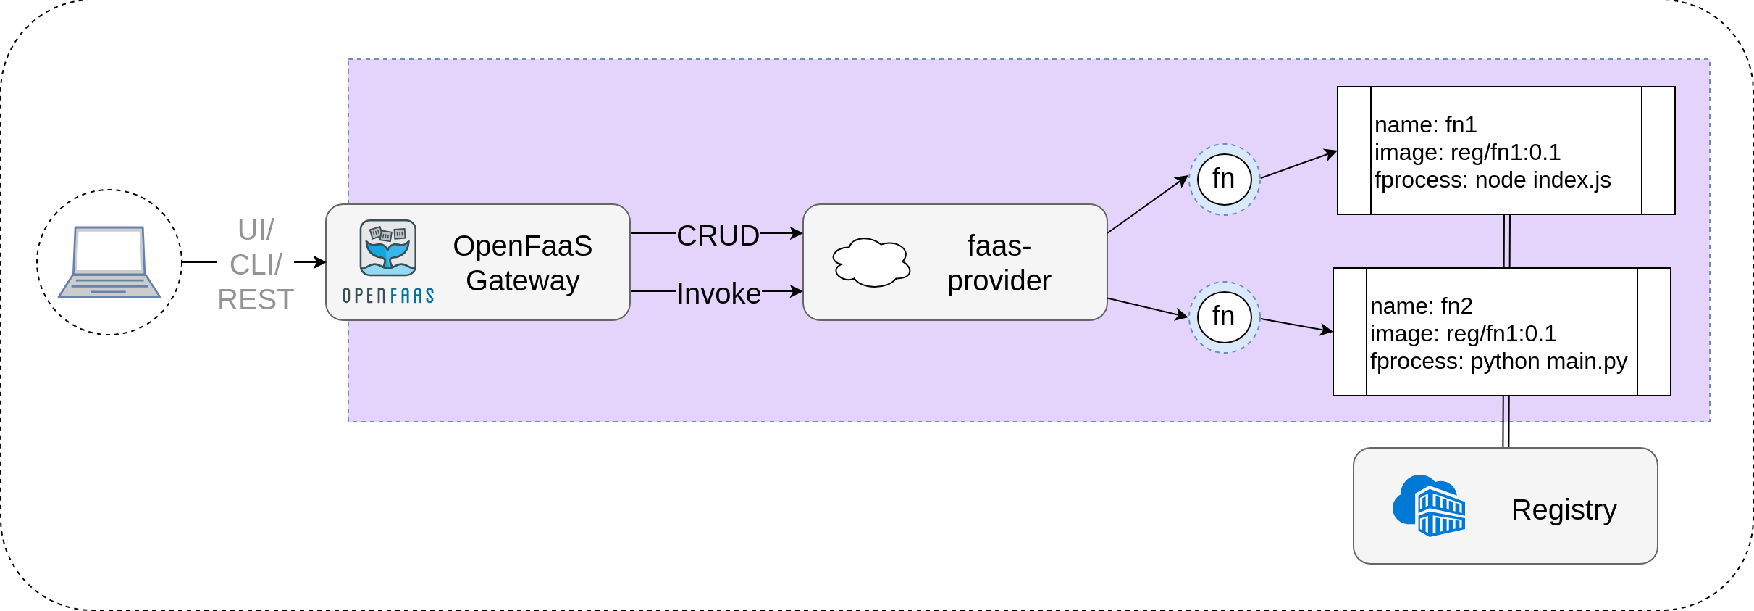
\includegraphics[width=\linewidth]{figures/OpenFaaS_provider.pdf}
    \caption{OpenFaaS Provider}
    \label{fig:openfaas-provider}
\end{figure}

\noindent
\underline{Kubernetes Provider:} \textbf{faas-netes} è il provider ufficiale per Kubernetes, impacchettato con \textit{Helm Charts}. Fornisce anche una \textit{Function \ac{crd}} tramite il flag \texttt{-operator=true}.

\subsubsection{faasd}

Si tratta di OpenFaaS senza la complessità ed il costo di Kubernetes. Questa soluzione richiede bassi requisiti, infatti esegue su un singolo host, ed è ampiamente compatibile con OpenFaaS su Kubernetes.
Sfrutta \textbf{containerd} e \textbf{\ac{cni}}, insieme ai componenti principali del progetto centrale.
\\
I casi d'uso principali sono:
\begin{itemize}
    \item esecuzione di codice localmente, usando container;
    
    \item creazione di automazione, portali web, bots, etc;
    
    \item ricerca di un modo per fare deployment remoti sopra \ac{rest} \ac{api};
    
    \item non si ha a disposizione larghezza di banda sufficiente per gestire Kubernetes;
    
    \item ``embedded apps" in \ac{IoT} e \textit{at the edge};
    
    \item costi ridotti;
    
    \item quando servono solo pochi microservizi o funzioni, senza il costo di un cluster.
\end{itemize}
Non comporta lo stesso onere di manutenzione che si ha con l'aggiornamento, il mantenimento e la gestione della sicurezza di un cluster Kubernetes.

\paragraph{\underline{Deployment}} ~\\
\textbf{faasd} è un binario statico che risiede in un sistema Linux configurato con \texttt{systemd} e richiede risorse di sistema minime.
\\
In base al sistema operativo ci sono delle differenze:
\begin{itemize}
    \item su Windows e MacOS si può usare \textit{multipass} per dispiegare \textit{faasd} in una \ac{vm};
    
    \item su Linux si può fare \texttt{deploy} direttamente o usare comunque \textit{multipass}.
\end{itemize}

\noindent
L'utilizzo per scopi di produzione richiede il \texttt{deploy} in uno dei seguenti modi:
\begin{itemize}
    \item uso dello script bash di installazione;
    
    \item utilizzo dello script \texttt{cloud-init} fornito;
    
    \item sfruttando Terraform\footnote{\url{https://www.terraform.io/}}.
\end{itemize}


\subsection{Knative}

Si tratta di un framework costruito sopra Kubernetes e Istio\footnote{\url{https://istio.io/}}; quindi estende la piattaforma di Kubernetes utilizzando le \acp{crd} per abilitare un livello di astrazione superiore. Tuttavia, non si può considerare una piattaforma serverless completa, dato che alcune implementazioni non vengono gestite, ma vengono lasciate allo sviluppatore, il quale talvolta può affidarsi ad altri framework per completare l'architettura.
Il framework, che viene mostrato nella \Cref{fig:architettura-knative}, è formato principalmente dai seguenti componenti:
\begin{itemize}
    \item \textbf{Serving}: definisce un insieme di oggetti come \textit{Kubernetes \acp{crd}}. Queste risorse sono usate per definire e controllare come si comporta il carico di lavoro serverless nel cluster. Come rappresentato nella \Cref{fig:architettura-knative-serving}, i componenti principali che lo compongono sono:
        \begin{itemize}
            \item \textbf{Services}: gestiscono automaticamente il ciclo di vita del carico di lavoro.
            
            \item \textbf{Routes}: gestiscono il traffico.
            
            \item \textbf{Configurations}: mantengono lo stato desiderato per il deployment.
            
            \item \textbf{Revisions}: sono oggetti immutabili che consistono in ``snapshots" del codice e della configurazione.
        \end{itemize}
        
    \begin{figure}[ht]
        \centering
        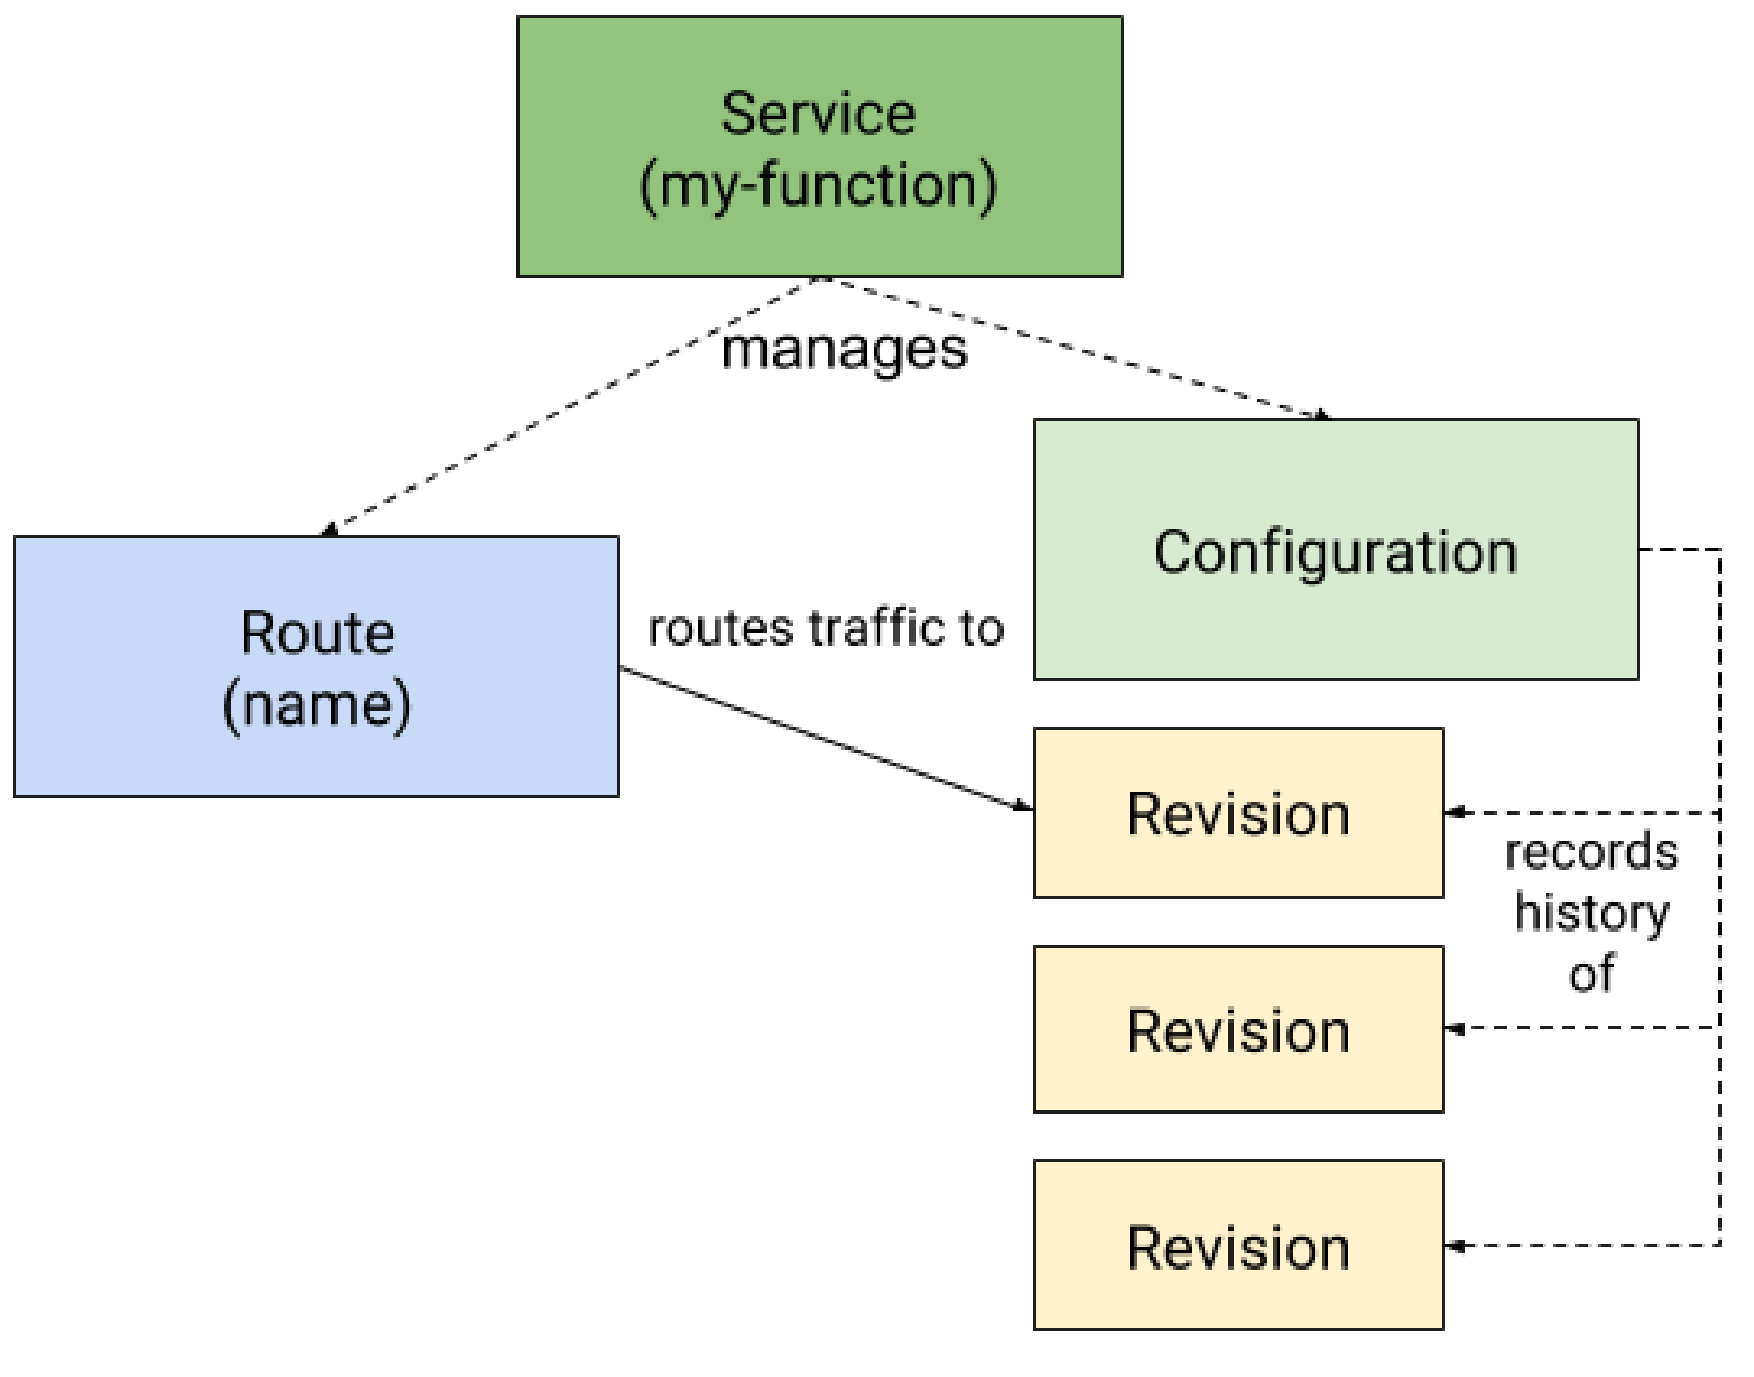
\includegraphics[width=0.9\linewidth]{figures/knative_serving.pdf}
        \caption{Architettura Knative Serving}
        \label{fig:architettura-knative-serving}
    \end{figure}
    
    \item \textbf{Eventing}: è una collezione di \ac{api} che consentono di usare un'architettura event-driven nelle applicazioni.
    Le principali caratteristiche sono le seguenti:
    \begin{itemize}
        \item le \ac{api} possono essere usate per creare componenti che instradano gli eventi dalle sorgenti (\textit{event producers}) ai consumatori (\textit{sinks});
        
        \item si tratta di una piattaforma a sé stante che fornisce supporto per vari carichi di lavoro;
        
        \item utilizza richieste di tipo \ac{http} POST per inviare e ricevere eventi tra sorgenti e \textit{sinks};
        
        \item i suoi componenti non sono molto legati, quindi possono essere sviluppati e dispiegati indipendentemente tra loro.
    \end{itemize}
\end{itemize}

\begin{figure}[ht]
    \centering
    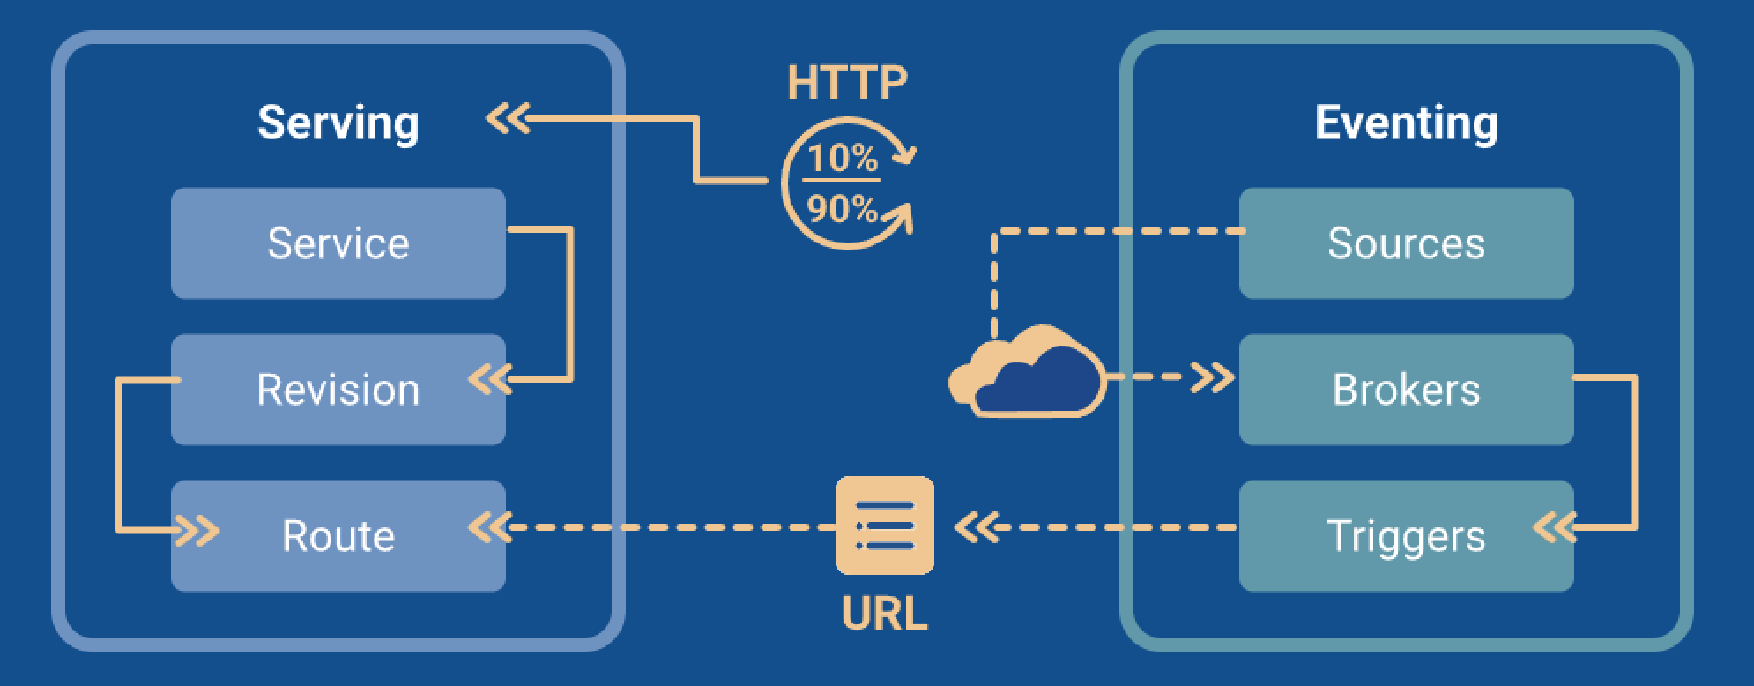
\includegraphics[width=\linewidth]{figures/knative_architecture.pdf}
    \caption{Architettura Knative}
    \label{fig:architettura-knative}
\end{figure}

\subsubsection{Knative Functions}

\textbf{Knative Functions} fornisce un semplice modello di programmazione per usare funzioni, senza la necessità di possedere una conoscenza approfondita di Kubernetes, \textit{Dockerfiles}, etc.
Esse inoltre abilitano la creazione, la costruzione e il \texttt{deploy} in modo semplice di funzioni stateless ed event-driven, sotto forma di \textbf{Knative Services}, sfruttando la \ac{cli} \textbf{func} o il relativo plugin \textbf{kn func}.
Quando si costruisce o esegue una funzione, un'immagine di container in formato \ac{oci} viene generata automaticamente e viene archiviata in un \textit{container registry}. Ogni volta che si aggiorna il codice e poi si esegue o viene fatto il \texttt{deploy}, allora anche l'immagine viene aggiornata.

\paragraph{\underline{Creazione funzione}} ~\\
Dopo aver installato \textit{Knative Functions} si può creare un progetto nel seguente modo:
\begin{lstlisting}
(kn) func create -l <language> <function-name>\end{lstlisting}

\paragraph{\underline{Esecuzione funzione}} ~\\
L'esecuzione di una funzione crea un'immagine di container in formato \ac{oci} per essa, prima di eseguirla in ambiente locale, ma non effettua il \texttt{deploy} su un cluster. Questo è utile se si vuole eseguire una funzione localmente per testarla.
\\ \\
\underline{Requisiti:}
\begin{itemize}
    \item si ha un \textbf{Docker daemon} in locale.
\end{itemize}

\noindent
\underline{Procedura:}
\\
Il comando \texttt{run} costruisce un'immagine per la funzione richiesta e la esegue localmente. Se non è ancora stata fatta la \texttt{build} della funzione allora è necessario il flag \texttt{--registry}.
Per eseguire la funzione localmente è necessario lanciare il seguente comando dall'interno della directory del progetto:
\begin{lstlisting}
(kn) func run [--registry <registry>]\end{lstlisting}


\paragraph{\underline{Deploy funzione}} ~\\
Fare il \texttt{deploy} di una funzione, come anticipato precedentemente, crea un'immagine di container \ac{oci} per la funzione ed effettua il \texttt{push} nell'\textit{image registry}. La funzione è dispiegata sul cluster come un \textit{Knative Service}.
In caso di reiterazione del \texttt{deploy} si aggiorna l'immagine ed il corrispondente \textit{Service} che è in esecuzione nel cluster. Le funzioni sul cluster sono accessibili come i servizi.
\\ \\
\underline{Requisiti:}
\begin{itemize}
    \item è presente un \textbf{Docker daemon} localmente;
    
    \item si ha accesso ad un \textit{container registry} ed è possibile fare il \texttt{push} delle immagini in esso.
\end{itemize}

\noindent
\underline{Procedura:}
\\
Il comando \texttt{deploy} usa il nome del progetto come nome del \textit{Knative Service}. Quando la funzione è costruita, il nome del progetto e il nome del registry sono usati per costruire un nome pienamente qualificato per l'immagine della funzione.
\begin{lstlisting}
(kn) func deploy --registry <registry>\end{lstlisting}


\paragraph{\underline{Build funzione}} ~\\
Costruire una funzione causa la creazione di un'immagine di container \ac{oci} per essa, la quale può subire poi il \texttt{push} nel registry. Questo comando non effettua il \texttt{deploy} e non esegue la funzione, il che è utile se si vuole costruire un'immagine localmente, ma non eseguirla o fare il \texttt{deploy} automaticamente al cluster.

\begin{enumerate}
    \item \textbf{Build locale}
        \\
        \underline{Requisiti:}
        \begin{itemize}
            \item si possiede un \textbf{Docker daemon} in locale.
        \end{itemize}

        \underline{Procedura:}
        \\
        Il comando \texttt{build} usa il nome del progetto e dell'\textit{image registry} per costruire un nome pienamente qualificato per l'immagine della funzione. Se il progetto non era già stato costruito bisogna fornire un \textit{image registry}.
        \begin{lstlisting}
(kn) func build\end{lstlisting}

    \item \textbf{Build on-cluster}
    \\
    \underline{Requisiti:}
        \begin{itemize}
            \item la funzione deve esistere in un repository Git\footnote{\url{https://git-scm.com/}};
            
            \item si deve configurare il cluster per usare \textit{Tekton Pipelines}.
        \end{itemize}

        \underline{Procedura:}
        \\
        La prima volta che si utilizza tale comando è indispensabile specificare l'\ac{url} di Git per la funzione:
        \begin{lstlisting}
(kn) func deploy --remote --registry <registry> --git-url <git-url> -p hello\end{lstlisting}
\end{enumerate}

\paragraph{\underline{Subscribe funzione a CloudEvents}} ~\\
\underline{Requisiti:}
\begin{itemize}
    \item \textbf{Knative Eventing} installato nel cluster.
\end{itemize}

\noindent
\underline{Procedura:}
\\
Il comando \texttt{subscribe} connette la funzione ad un gruppo di eventi, rispettando una serie di filtri per \textit{Cloud Event metadata} e \textit{Knative Broker}, come fonti di eventi.
\\
Quando si iscrive una funzione ad alcuni eventi per un \textit{broker}, se non specificato, si considera quello di default:
\begin{lstlisting}
(kn) func subscribe --filter type=com.example --filter extension=my-extension-value [--source my-broker]\end{lstlisting}

\paragraph{\underline{Invocazione funzione}} ~\\
Con il seguente comando si invia una richiesta di test per invocare una funzione localmente o nel cluster: \begin{lstlisting}
(kn) func invoke\end{lstlisting}

\noindent
Questo comando viene usato per testare che una funzione non abbia problemi e sia in grado di ricevere correttamente richieste \ac{http} e \textbf{CloudEvents}.
\\
Ci sono vari tipi di flag per simulare diverse tipologie di richieste, per esempio aggiungendo il flag \texttt{--data} si possono inviare dati di test alla funzione.
\\
In alternativa, è possibile invocare una funzione inviando richieste \ac{http} (per esempio tramite il comando \texttt{curl}) all'indirizzo fornito a seguito del \texttt{deploy} della funzione, messo a disposizione da \textit{Knative Serving}.

%You may also put some code snippet (which is NOT float by default), eg: \cref{lst:random-code}.

%\lstinputlisting[language=Java,label={lst:random-code}]{listings/HelloWorld.java}

%\section{Fancy formulas here}

%----------------------------------------------------------------------------------------
\chapter{Setup sperimentale}
\label{chap:setup-sperimentale}
%----------------------------------------------------------------------------------------

L'analisi dei framework \textbf{Knative}, \textbf{OpenWhisk} e \textbf{OpenFaaS} è stata realizzata sopra un'architettura sperimentale, la quale è formata da due strati (``layer"):
\begin{itemize}
    \item \textbf{strato fisico}: composto da una macchina fisica equipaggiata con una CPU \\
    \texttt{Intel(R) Core(TM) i5-11300H 4.40GHz} e \texttt{8GB di RAM DDR4 3200MHz}. Il sistema operativo della macchina è \texttt{Kubuntu 22.04.4 LTS}.
    
    \item \textbf{strato virtualizzato}: nel quale la macchina fisica ha installato Docker in versione \texttt{v27.2.0}. I container sono gestiti tramite Kubernetes, ovvero un sistema di orchestrazione e gestione di container, il quale è presente all'interno del dispositivo nella versione \texttt{v1.31.0}. È stato creato un cluster per ogni framework, formato da un unico \textit{control plane}, tramite il tool KinD, il quale consente di eseguire cluster Kubernetes localmente, sfruttando i container Docker come nodi.
\end{itemize}
Si è utilizzata la medesima macchina fisica per inviare richieste \ac{http}, con lo scopo di invocare le funzioni di cui si era fatto il \texttt{deploy} su ogni framework serverless. Questo processo di test è stato realizzato mediante una procedura per verificare il comportamento dei framework in diverse situazioni di distribuzione del carico e gestito grazie all'applicazione \textbf{JMeter}\footnote{\url{https://jmeter.apache.org/}}. Le modalità di autoscaling suddivise per framework, le quali vengono ulteriormente analizzate nel seguente articolo~\cite{Li2021}, in particolare OpenFaaS e Knative, sono:
\begin{itemize}
    \item \textbf{OpenFaaS}: il componente \textit{AlertManager} legge le metriche (richieste per secondo) dal componente \textit{Prometheus}, in modo da sapere quando inviare un avviso all'\textit{API gateway}.
    
    \item \textbf{Knative}: si è optato per il \textbf{\ac{kpa}}, che è una parte di \textit{Knative Serving}, tramite il quale si effettua un autoscaling in base alle richieste per secondo.
    
    \item \textbf{OpenWhisk}: mette a disposizione la possibilità di utilizzare l'\textit{autoscaler} di Kubernetes, come l'\ac{hpa}.
\end{itemize}

\section{Metriche qualitative}
\label{sec:metriche-qualitative}

Le metriche qualitative prese in considerazione per confrontare le diverse piattaforme, sono:
\begin{itemize}
    \item linguaggi di programmazione supportati;
    
    \item supporto a orchestratori di container;
    
    \item supporto al monitoraggio: ovvero possedere uno strumento di monitoraggio integrato per controllare ed analizzare le performance;
    
    \item modalità di invocazione: nello specifico supporto ad invocazioni sincrone (\textit{\ac{http}-based}) ed asincrone (\textit{event-based});
    
    \item interfaccia \ac{cli}.
\end{itemize}


\section{Metriche quantitative}
\label{sec:metriche-quantitative}

Lo scopo è quello di verificare l'efficienza nella scalabilità in base al carico; dunque si considerano le seguenti metriche:
\begin{itemize}
    \item \textbf{tempo di risposta}: il tempo di risoluzione della richiesta. Viene presa in considerazione la sua misura media in millisecondi;
    
    \item \textbf{throughput}: il numero di richieste soddisfatte per secondo. L'unità di misura utilizzata è il numero di transazioni al secondo;
    
    \item \textbf{tasso di successo}: il rapporto tra il numero di richieste con esito positivo e il numero di richieste totali; considerato in percentuale.
\end{itemize}
Queste metriche vengono testate tramite il tool JMeter, il quale è stato configurato per eseguire 10 richieste \ac{http} con vari livelli di concorrenza (nello specifico 1, 5, 10, 15 e 20), ovvero il numero di utenti da simulare contemporaneamente. Quest'ultimo viene specificato in JMeter tramite il valore \textit{Number of Threads (Users)}, richiesto durante la creazione di un \textit{Thread Group}. Questo è stato fatto per ogni framework e a sua volta per tutte le funzioni: Node.js, Python e Java.


%----------------------------------------------------------------------------------------
\chapter{Creazione sistema di test}
\label{chap:creazione-sistema-test}
%----------------------------------------------------------------------------------------

È stato creato un sistema di test per verificare l'effettivo funzionamento dei seguenti framework: \textbf{Knative}, \textbf{Apache OpenWhisk} e \textbf{OpenFaaS}. Per ogni framework si riportano i passaggi necessari per la configurazione e le modalità di testing delle funzioni.
Il test è stato eseguito per tre linguaggi diversi: Python, Node.js e Java. Tutte le funzioni implementano la stessa logica, poco dispendiosa in termini di risorse: ricevono in input un file \texttt{JSON} e restituiscono una risposta nello stesso formato, che comprende:
\begin{itemize}
    \item dati presenti nel file;
    
    \item numero di elementi presenti nel file;
    
    \item dimensione del file (in Bytes).
\end{itemize}
Le differenze nelle tre funzioni riguardano principalmente le specificità richieste dal linguaggio, come per esempio le funzioni messe a disposizione per la gestione del formato \texttt{JSON}.
\\
La fase di test che si vuole realizzare consiste nell'osservare il comportamento del framework di fronte ad un carico di lavoro, il quale può variare in base alle richieste ricevute; inoltre realizzando la funzione in tre linguaggi diversi, si è in grado di notare se la scelta di un linguaggio rispetto ad un altro incide nelle prestazioni.

\paragraph{\underline{Creazione test}} ~\\
I test sono stati creati, come detto in precedenza, tramite JMeter, grazie al quale è stato possibile realizzarne uno per ogni linguaggio ed ogni livello di concorrenza.
Il software consente di creare dei test aggiungendo un \textbf{Thread Group} con alcuni parametri:
\begin{itemize}
    \item \textbf{Number of Threads (Users)}: determina il numero di utenti da simulare contemporaneamente; viene utilizzato dunque per configurare il livello di concorrenza. Questo parametro in ogni test assume un valore diverso tra 1, 5, 10, 15 e 20.
    
    \item \textbf{Ramp-up period (seconds)}: specifica la durata della piena attività degli utenti, mentre JMeter avvia i thread. Questo valore viene scelto sempre uguale ad un secondo, in questo modo si dice a JMeter che in questo intervallo di tempo deve aver avviato tutti i thread.
    
    \item \textbf{Loop Count}: indica quante volte i thread eseguiranno il test, dunque questo valore viene impostato sempre uguale a 10, in modo da effettuare le richieste \ac{http} prefissate.
\end{itemize}
Successivamente al \textit{Thread Group} si aggiunge una richiesta \ac{http} opportunamente configurata come segue:
\begin{itemize}
    \item si inserisce il protocollo da utilizzare (\ac{http}/\ac{https});
    
    \item si inserisce l'\ac{url} per raggiungere la funzione da testare;
    
    \item si sceglie il metodo della richiesta; quindi in questo caso il metodo POST;
    
    \item si aggiunge il file \texttt{JSON} da passare come argomento.
\end{itemize}

\noindent
I test per il framework Apache OpenWhisk richiedono anche l'aggiunta, nella richiesta \ac{http}, di un \textit{Authorization Manager}; all'interno del quale si specificano l'\textit{\ac{api} Host} e l'\textit{Authentication Key}, impostati durante la fase di installazione, per l'\ac{url} al quale si inviano le richieste. Inoltre, il suddetto framework è anche l'unico al quale vengono fatte richieste con il protocollo \ac{https}, motivo per cui è necessario fornire l'autorizzazione per accedere alle risorse.

\paragraph{\underline{Svolgimento test}} ~\\
Per eseguire i test si è sfruttato il seguente comando da \ac{cli}, in questo modo si limitano al massimo le risorse occupate da altri processi, come la \ac{gui} di JMeter:
\begin{lstlisting}
jmeter -n -t <path-to-file>/test.jmx -l <path-to-file>/test.csv -e -o
<path-to-directory>/test_report.html\end{lstlisting}
Questo comando specifica il file \texttt{.jmx}, che consiste nel test creato con JMeter; inoltre si specificano un file \texttt{csv} e una directory, all'interno dei quali verranno inseriti i risultati del test.
\\ \\
Gli esperimenti effettuati e il procedimento per poterli replicare si possono trovare nell'apposito repository\footnote{\url{https://github.com/FilippoPracucci/FaaS_frameworks}}.


%----------------------------------------------------------------------------------------
\chapter{Risultati sperimentali}
\label{chap:risultati-sperimentali}
%----------------------------------------------------------------------------------------

\begin{table}
    \centering
    \begin{tabularx}{\linewidth} {
  | >{\centering\arraybackslash}X 
  | >{\centering\arraybackslash}X
  | >{\centering\arraybackslash}X
  | >{\centering\arraybackslash}X | }
        \hline
          &  \textbf{OpenFaaS} & \textbf{Knative} & \textbf{Apache OpenWhisk} \\ [0.8ex]
        \hline
        \textbf{Linguaggi di programmazione supportati} & Bash, Dockerfile, C\#, Go, Java, Node.js, PHP, Python, Ruby, Rust & Node.js, Python, Go, Quarkus, Rust, Spring Boot, TypeScript & Go, Java, Node.js, PHP, Python, Ruby, Rust, Swift, .NET Core, Dockerfile \\
        \hline
        \textbf{Supporto a Orchestratori di container} & Kubernetes, OpenShift\footnote{\url{https://www.redhat.com/it/technologies/cloud-computing/openshift}} & Kubernetes & Kubernetes, ``Standalone OpenWhisk Stack", Docker Compose, Ansible, Vagrant \\
        \hline
        \textbf{Supporto al monitoraggio} & Prometheus con Grafana\footnote{\url{https://grafana.com/}} & Prometheus con Grafana, OpenTelemetry Collector\footnote{\url{https://opentelemetry.io/docs/collector/}} & Nessuno \\
        \hline
        \textbf{Modalità di invocazione} & \ac{http} e sorgenti di eventi & \ac{http} e \textit{CloudEvents} & \ac{http} e \textit{Triggers} \\
        \hline
        \textbf{Interfaccia \ac{cli}} & faas-cli & kn, func & wsk \\
        \hline
    \end{tabularx}
    \caption{Metriche qualitative}
    \label{tab:tabella-metriche-qualitative}
\end{table}

La \Cref{tab:tabella-metriche-qualitative} mostra le valutazioni delle metriche qualitative citate nella \cref{sec:metriche-qualitative}. I risultati mostrano che i tre framework analizzati nel dettaglio offrono funzionalità comparabili. Per quanto riguarda le metriche quantitative, elencate nella \cref{sec:metriche-quantitative}, i risultati vengono mostrati nelle sezioni a seguire.

\section{Grafici risultati sperimentali Node.js}

In questa sezione si mostrano i grafici con i risultati dei test eseguiti per le funzioni Node.js. I grafici vengono suddivisi per metrica valutata e in ogni grafico si confrontano i risultati di tutti i framework. Quindi nella \Cref{fig:grafici-throughput-node} si mostrano le misurazioni riguardanti lo throughput, inteso come transazioni al secondo; nella \Cref{fig:grafici-tempo-risposta-node} si riportano i risultati riguardanti la metrica del tempo di risposta medio, in millisecondi, mentre nella \Cref{fig:grafici-tasso-successo-node} si visualizza il tasso di successo delle richieste. Infine, ogni grafico suddivide i risultati per livello di concorrenza del test.

\begin{figure}[ht]
    \centering
    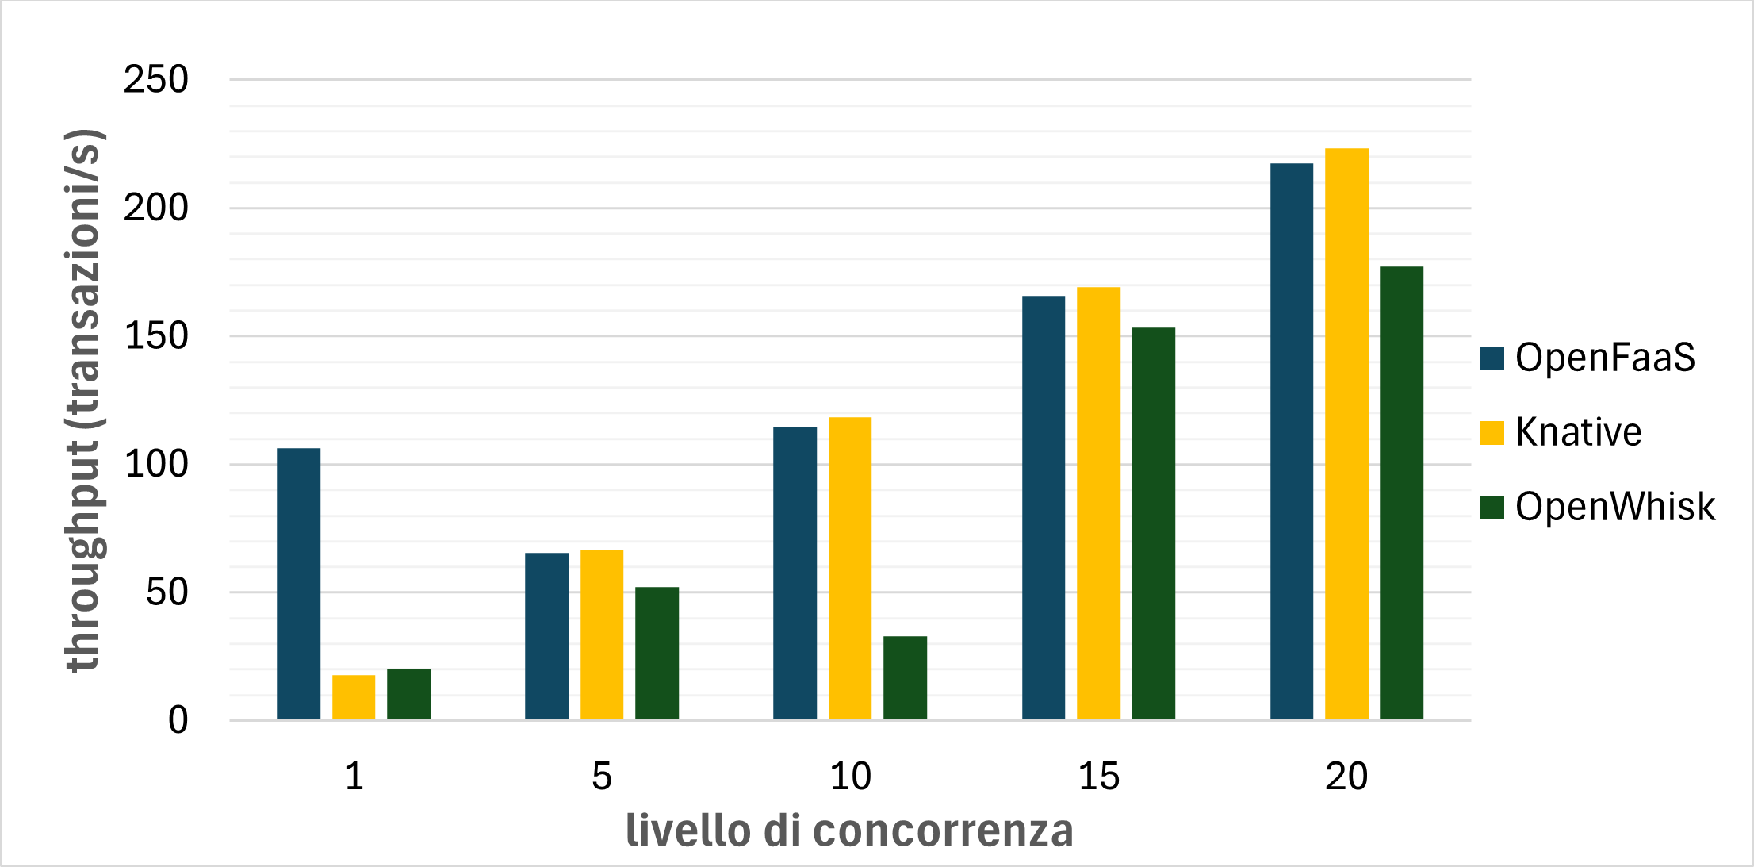
\includegraphics[width=0.95\linewidth]{figures/graphs/throughput_node.pdf}
    \caption{Grafici risultati sperimentali throughput (transazioni/s) Node.js}
    \label{fig:grafici-throughput-node}
\end{figure}

\begin{figure}[ht]
    \centering
    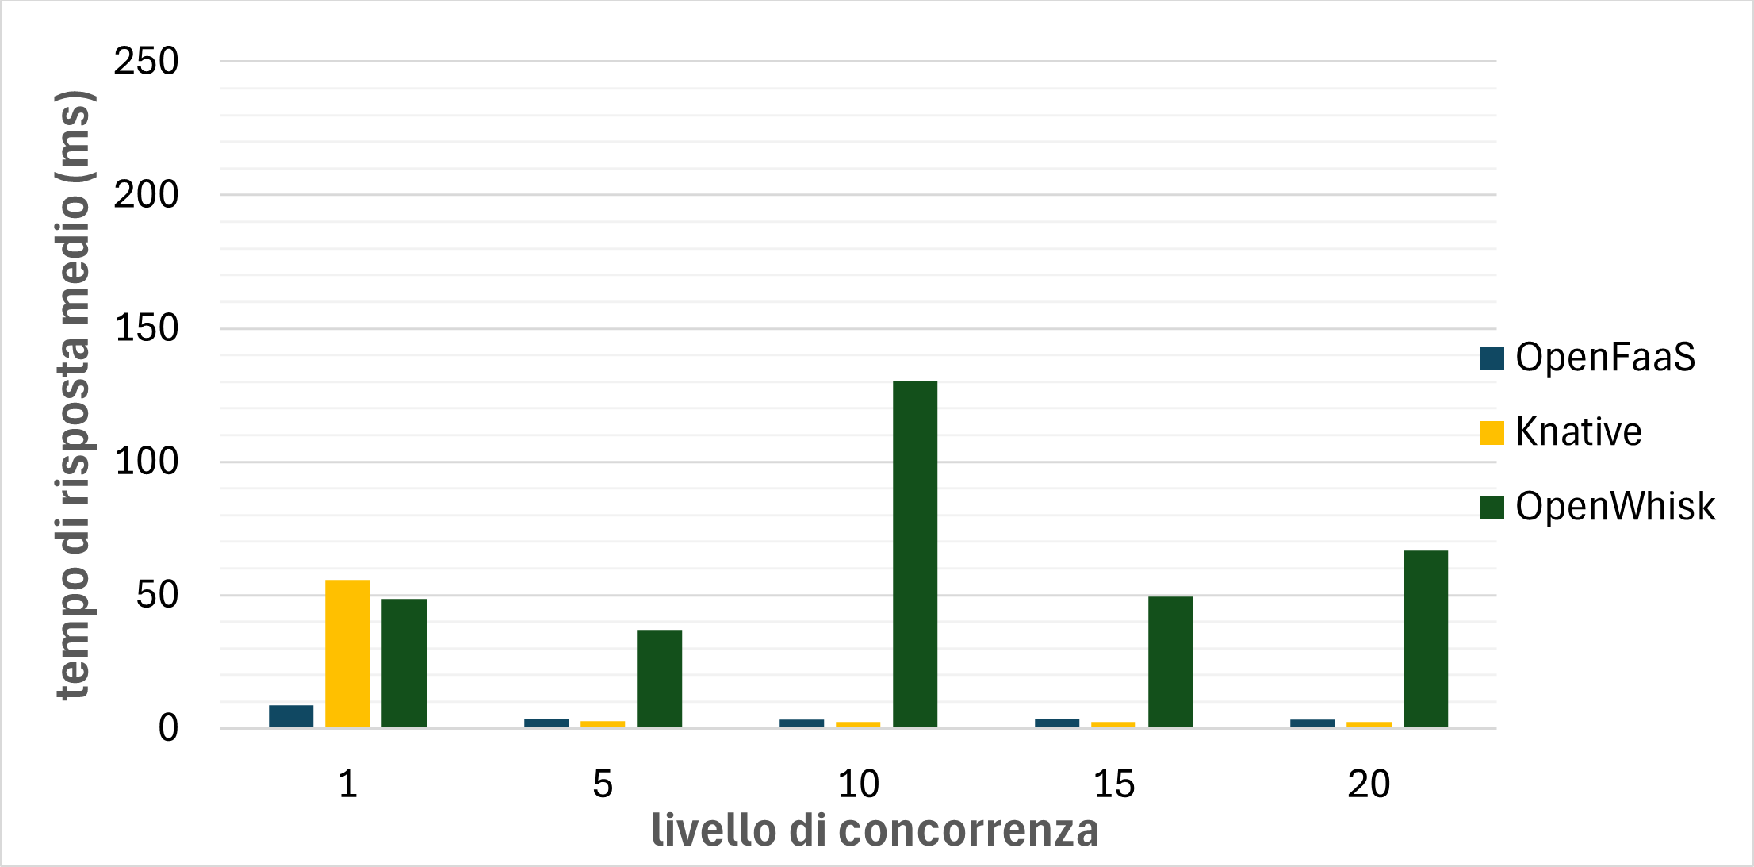
\includegraphics[width=0.95\linewidth]{figures/graphs/tempoRisposta_node.pdf}
    \caption{Grafici risultati sperimentali tempo di risposta medio (ms) Node.js}
    \label{fig:grafici-tempo-risposta-node}
\end{figure}

\begin{figure}[ht]
    \centering
    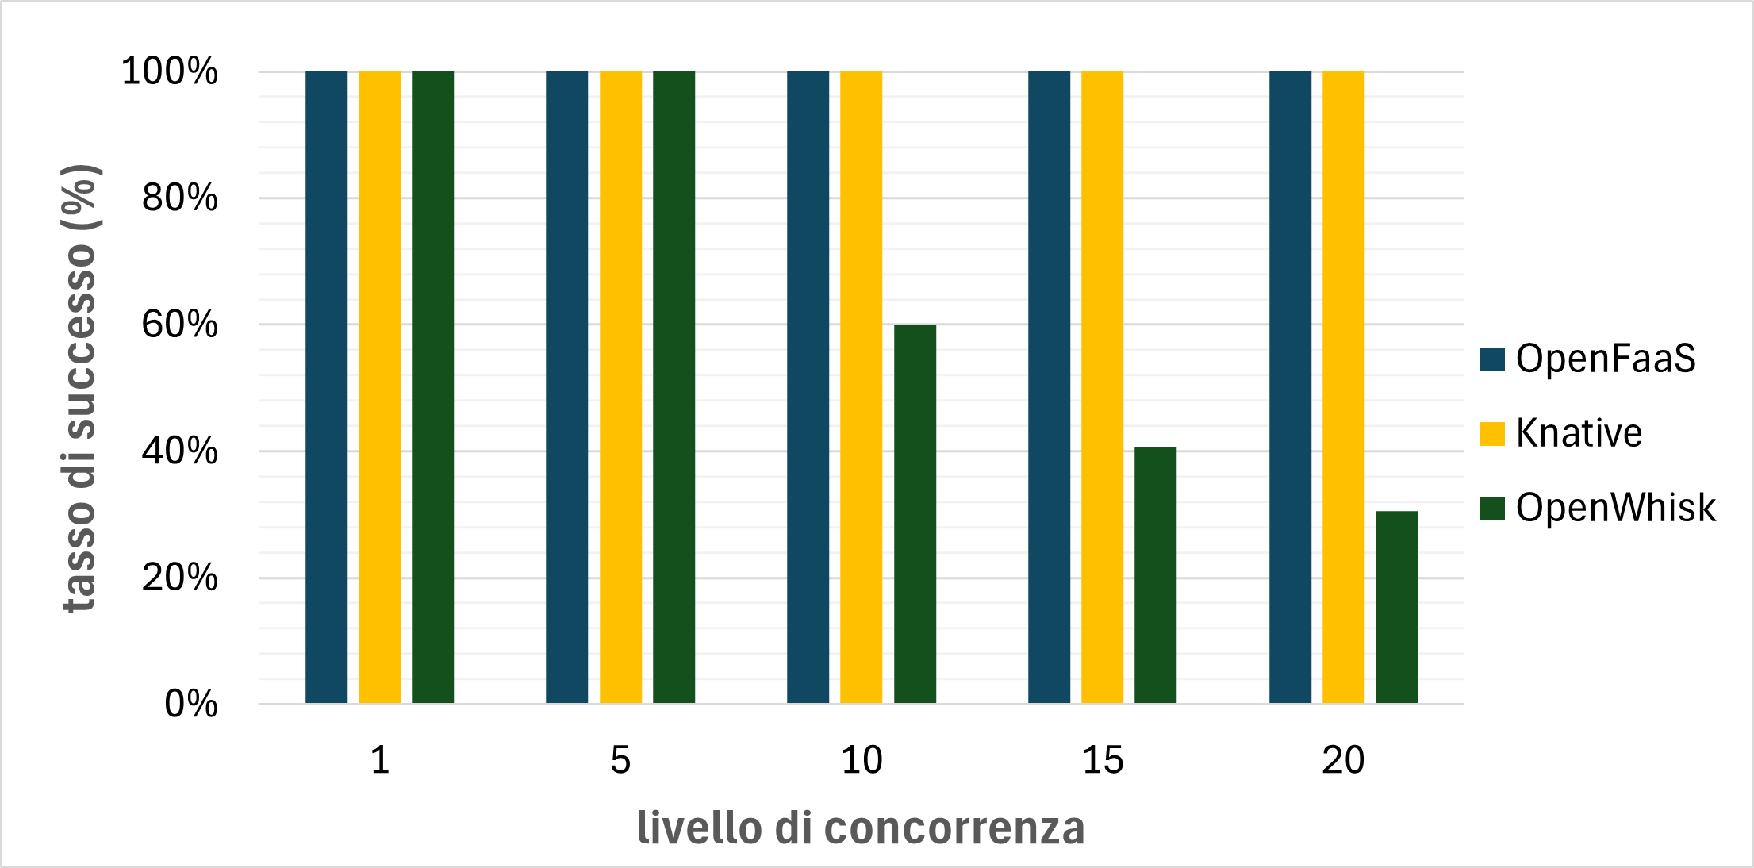
\includegraphics[width=0.95\linewidth]{figures/graphs/tassoSuccesso_node.pdf}
    \caption{Grafici risultati sperimentali tasso di successo (\%) Node.js}
    \label{fig:grafici-tasso-successo-node}
\end{figure}


\section{Grafici risultati sperimentali Python}

Si mostrano i grafici con i risultati dei test eseguiti per le funzioni Python. I grafici vengono suddivisi per metrica ed in ogni grafico si confrontano i risultati di ogni framework. Dunque nella \Cref{fig:grafici-throughput-python} si riporta lo throughput, inteso come transazioni al secondo; nella \Cref{fig:grafici-tempo-risposta-python} si mostrano i risultati riguardanti il tempo di risposta medio in millisecondi ed infine nella \Cref{fig:grafici-tasso-successo-python} si visualizza il tasso di successo delle richieste, in percentuale. Inoltre, ogni grafico suddivide i confronti per livello di concorrenza del test.

\begin{figure}[ht]
    \centering
    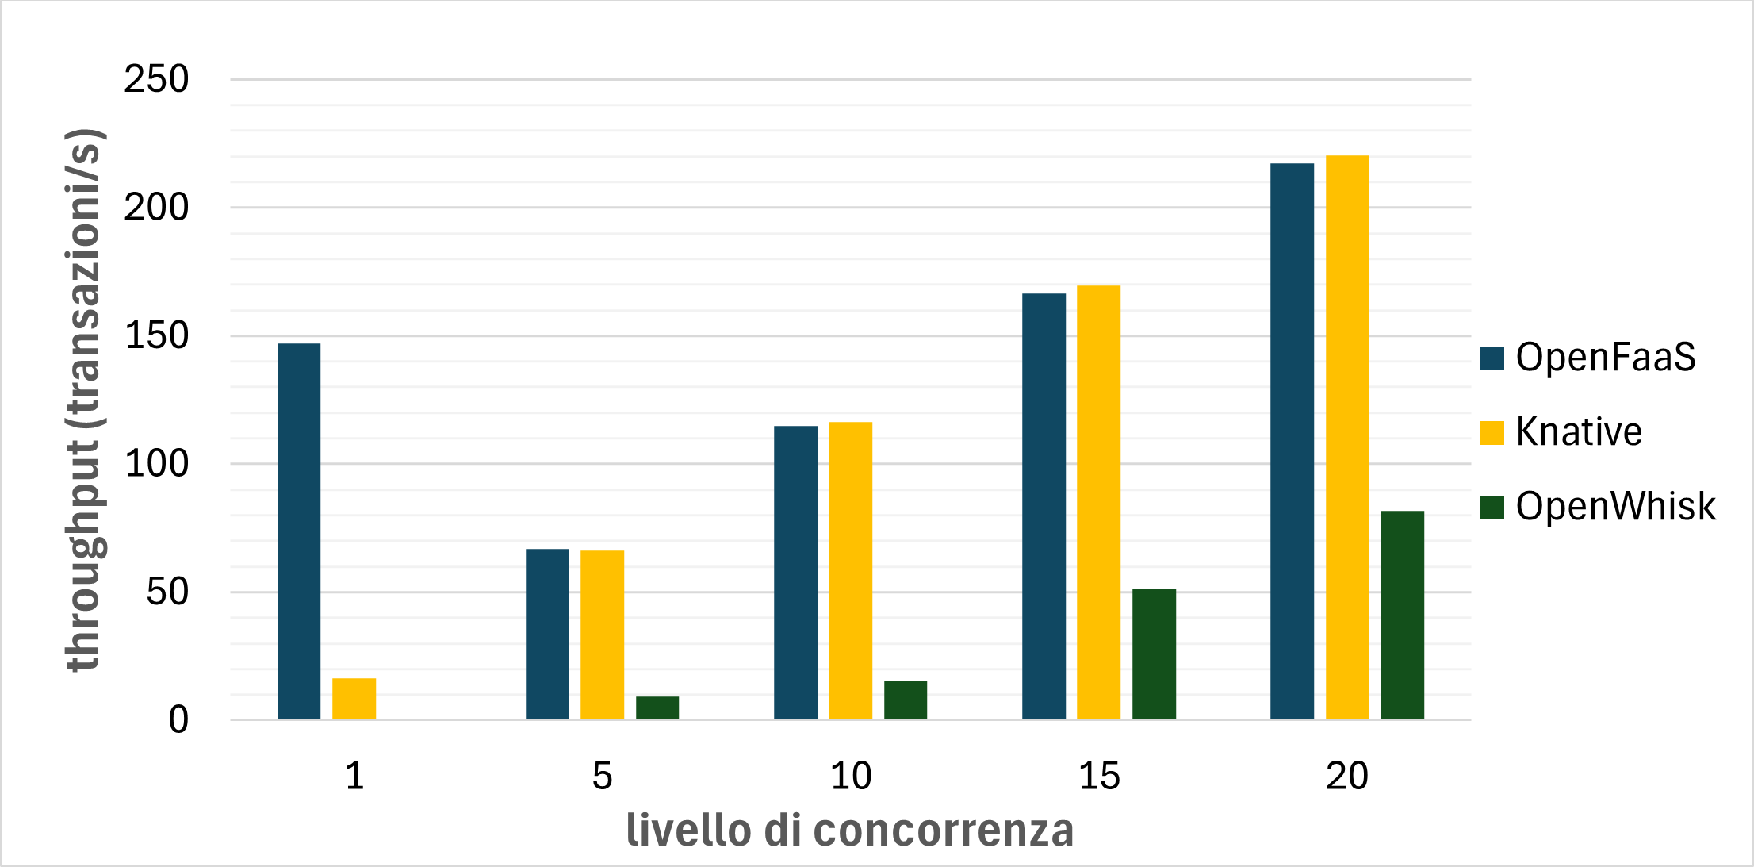
\includegraphics[width=0.95\linewidth]{figures/graphs/throughput_python.pdf}
    \caption{Grafici risultati sperimentali throughput (transazioni/s) Python}
    \label{fig:grafici-throughput-python}
\end{figure}

\begin{figure}[ht]
    \centering
    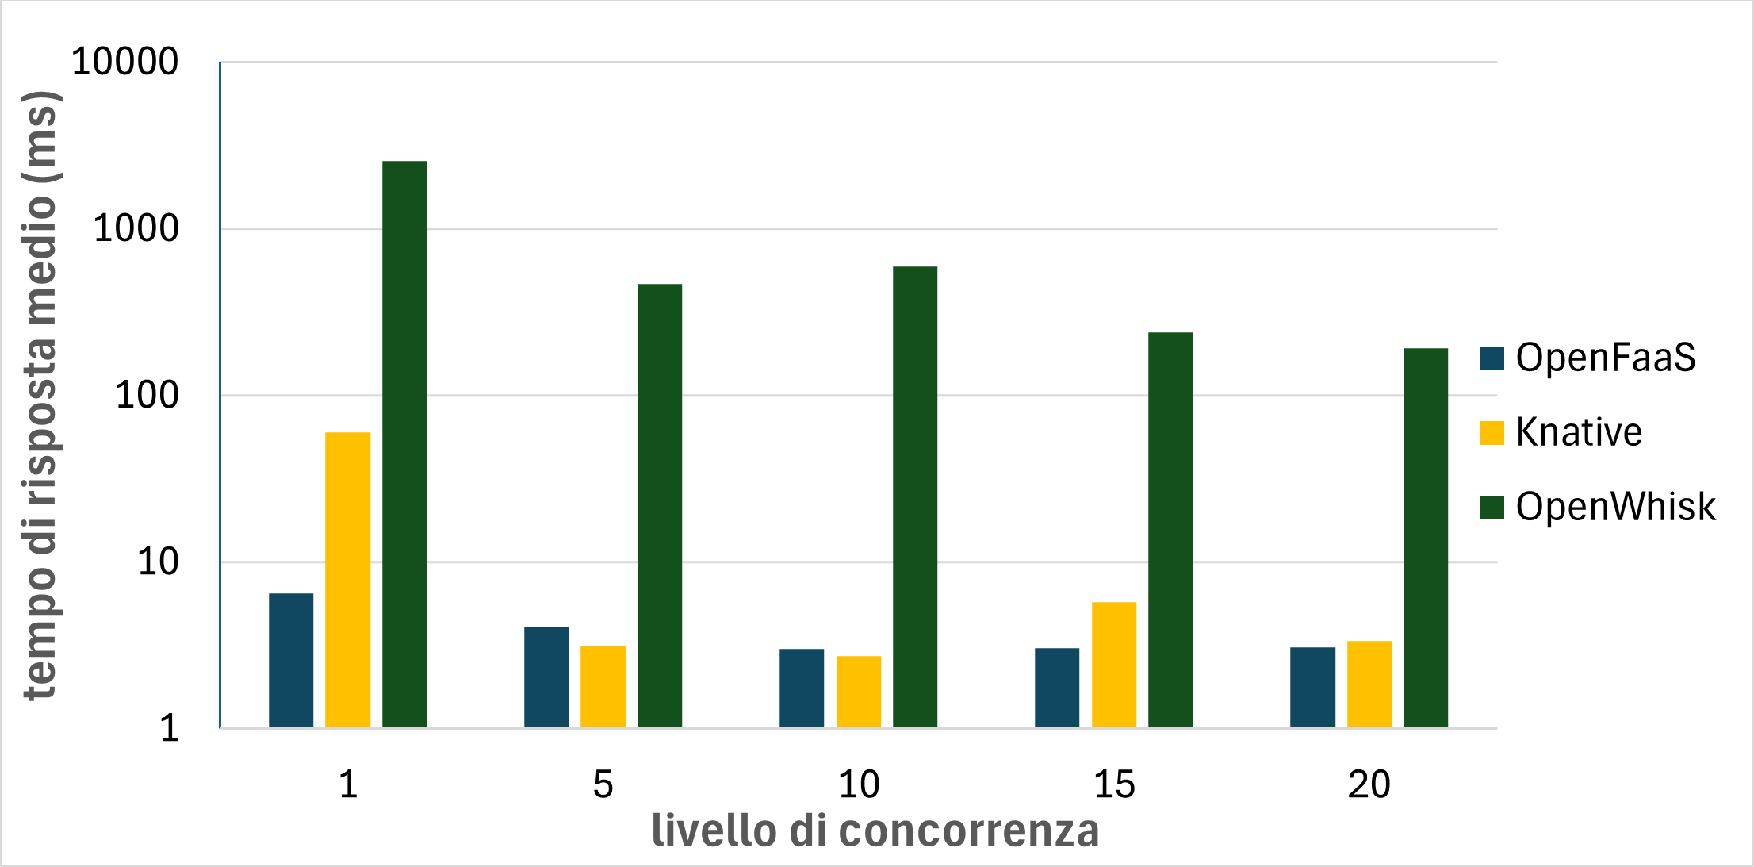
\includegraphics[width=0.95\linewidth]{figures/graphs/tempoRisposta_python.pdf}
    \caption{Grafici risultati sperimentali tempo di risposta medio (ms) Python}
    \label{fig:grafici-tempo-risposta-python}
\end{figure}

\begin{figure}[ht]
    \centering
    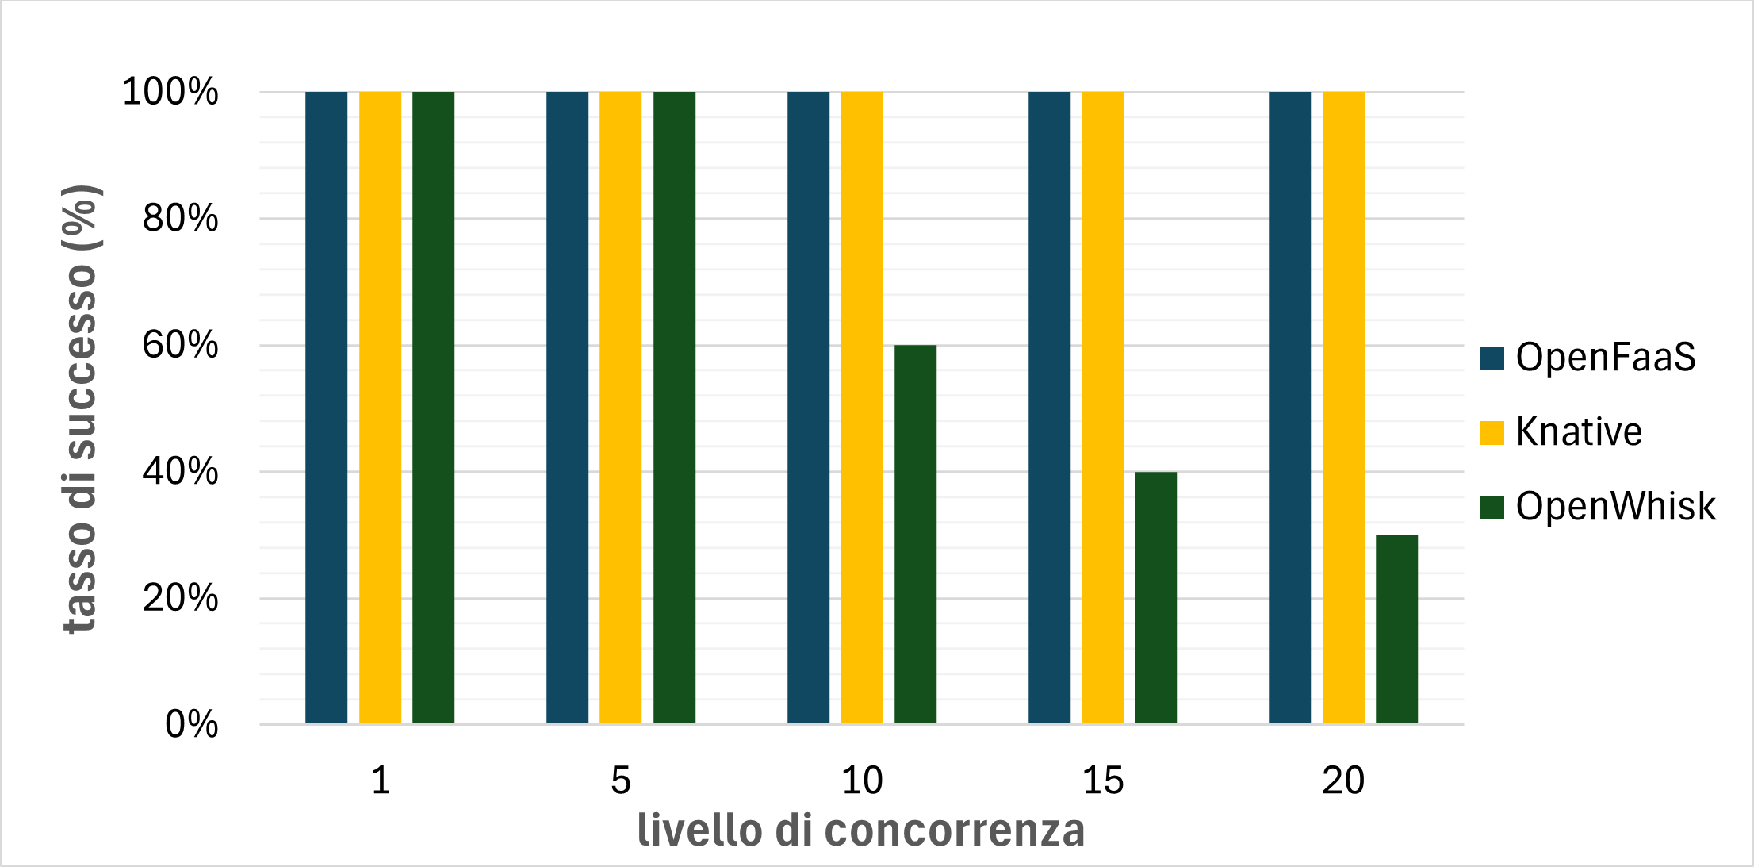
\includegraphics[width=0.95\linewidth]{figures/graphs/tassoSuccesso_python.pdf}
    \caption{Grafici risultati sperimentali tasso di successo (\%) Python}
    \label{fig:grafici-tasso-successo-python}
\end{figure}


\section{Grafici risultati sperimentali Java}

In questa sezione si mostrano i grafici rappresentanti i risultati dei test eseguiti per le funzioni Java. I grafici vengono separati in base alla metrica presa in considerazione per poi confrontare i risultati di tutti i framework. Nella \Cref{fig:grafici-throughput-java} si mostrano le misurazioni riguardanti la metrica dello throughput, misurata in transazioni al secondo; mentre nella \Cref{fig:grafici-tempo-risposta-java} si visualizzano i risultati relativi al tempo di risposta medio, in millisecondi ed infine nella \Cref{fig:grafici-tasso-successo-java} si riporta il tasso di successo delle richieste. Tutti i grafici suddividono i risultati in base al livello di concorrenza del test.

\begin{figure}[ht]
    \centering
    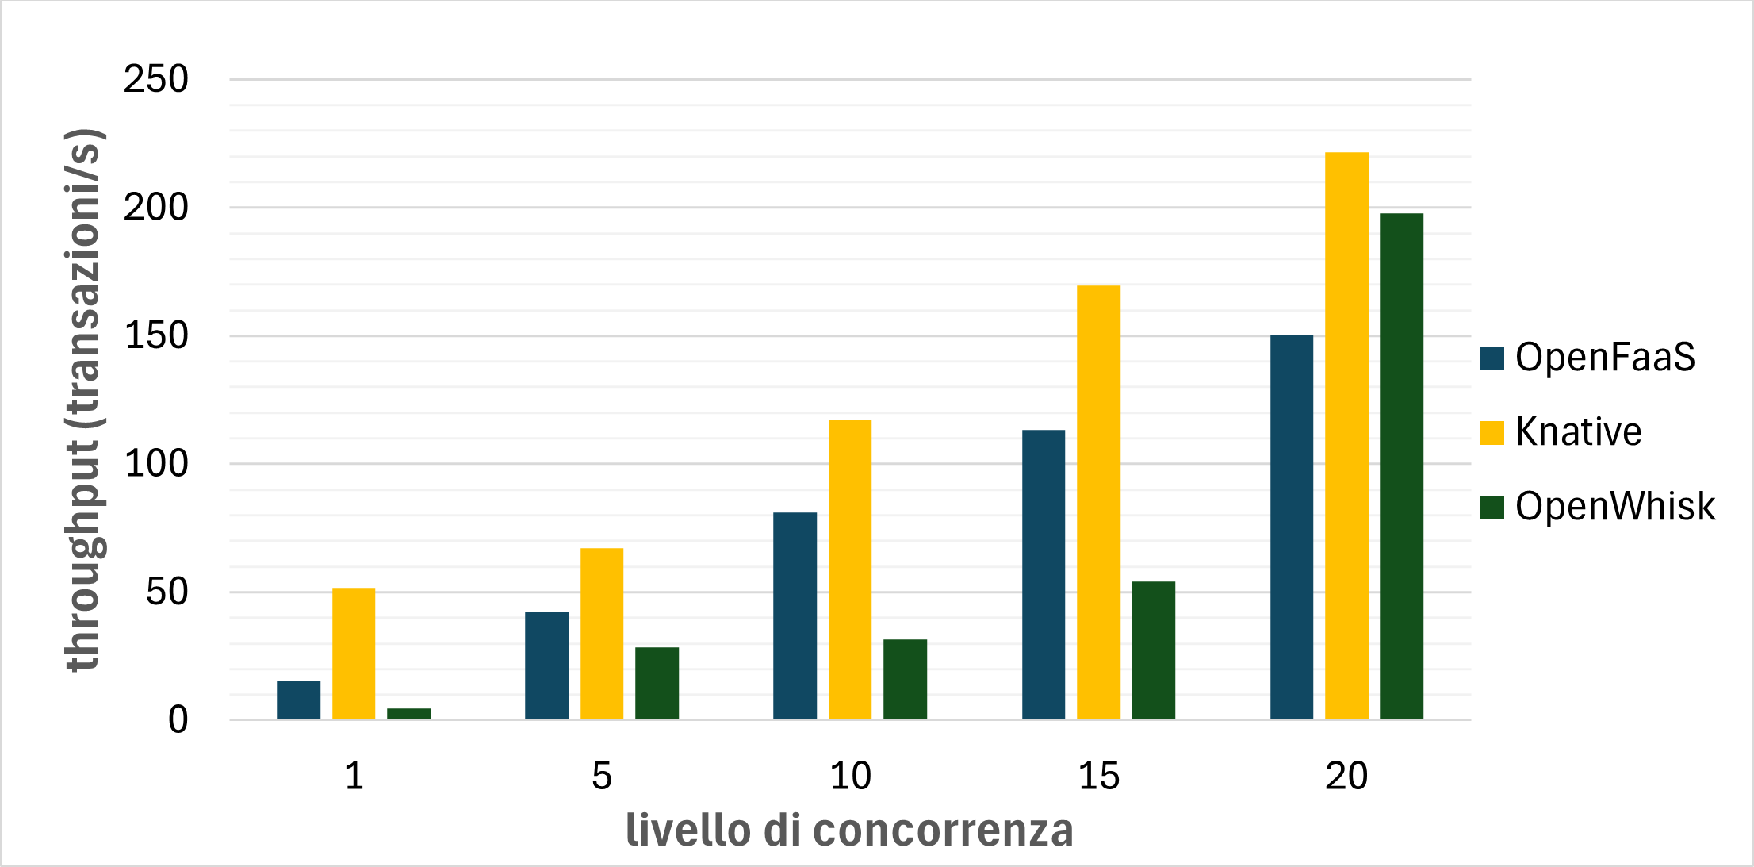
\includegraphics[width=0.95\linewidth]{figures/graphs/throughput_java.pdf}
    \caption{Grafici risultati sperimentali throughput (transazioni/s) Java}
    \label{fig:grafici-throughput-java}
\end{figure}

\begin{figure}[ht]
    \centering
    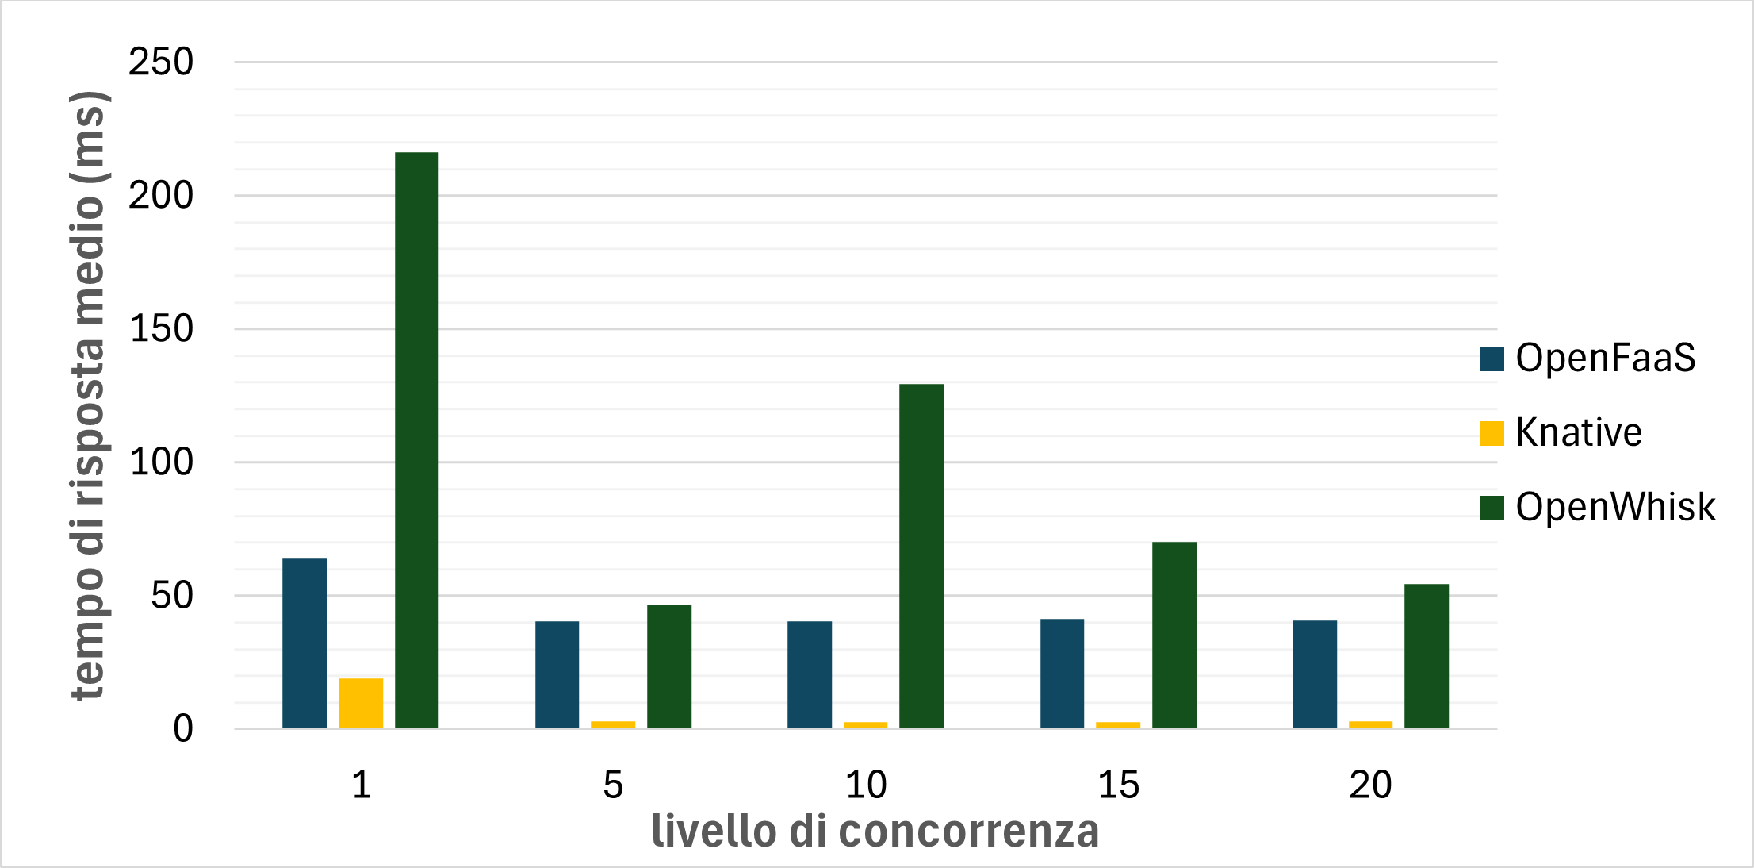
\includegraphics[width=0.95\linewidth]{figures/graphs/tempoRisposta_java.pdf}
    \caption{Grafici risultati sperimentali tempo di risposta medio (ms) Java}
    \label{fig:grafici-tempo-risposta-java}
\end{figure}
    
\begin{figure}[ht]
    \centering
    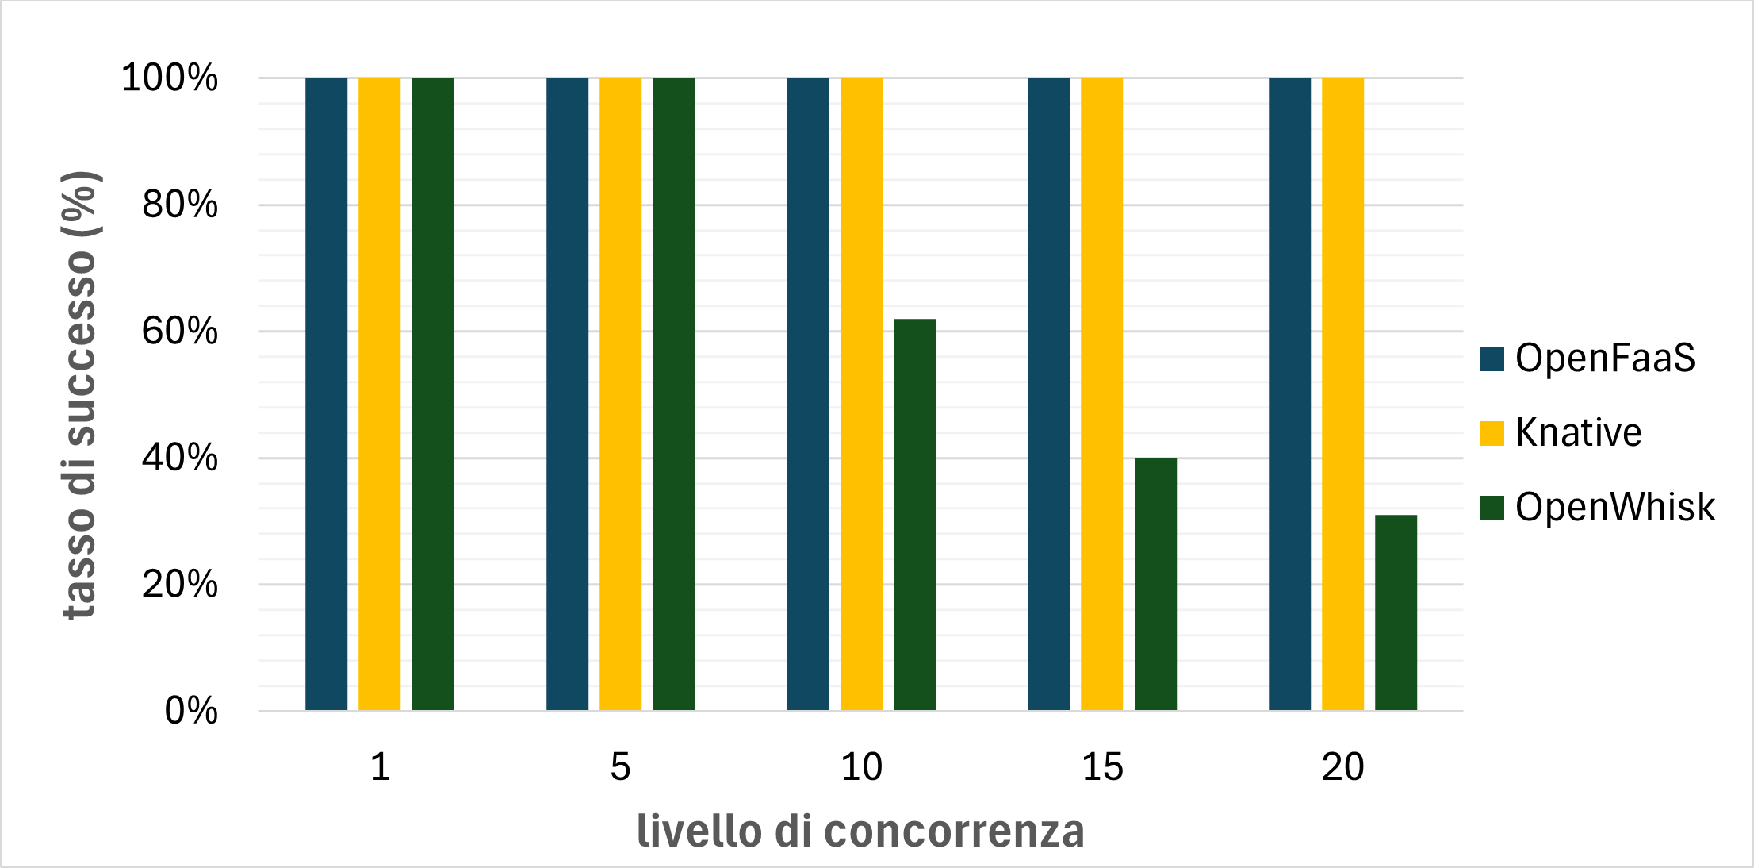
\includegraphics[width=0.95\linewidth]{figures/graphs/tassoSuccesso_java.pdf}
    \caption{Grafici risultati sperimentali tasso di successo (\%) Java}
    \label{fig:grafici-tasso-successo-java}
\end{figure}


\section{Analisi risultati}

I risultati che sono stati riportati nei grafici evidenziano vari aspetti:
\begin{itemize}
    \item OpenFaaS risulta essere il framework con prestazioni migliori sotto il punto di vista dello throughput. Infatti, come si può notare nelle  \Cref{fig:grafici-throughput-node} e \Cref{fig:grafici-throughput-python}, in corrispondenza delle funzioni realizzate in Node.js e Python, il suddetto framework mostra un numero di transazioni al secondo nettamente superiore rispetto agli altri con un livello di concorrenza uguale ad uno, per poi allinearsi ad essi all'aumentare del carico, in particolare con Knative. Il comportamento è diverso per la funzione realizzata in Java, il cui grafico è raffigurato nella \Cref{fig:grafici-throughput-java}, il quale evidenzia che lo throughput maggiore lo si ha in Knative per tutti i livelli di concorrenza. Questo è dovuto al fatto che il framework supporta tale linguaggio tramite l'ausilio dei framework Spring Boot\footnote{\url{https://spring.io/projects/spring-boot}} e Quarkus\footnote{\url{https://quarkus.io/}} (in questo caso è stato sfruttato il primo). In generale, all'aumentare del livello di concorrenza, lo throughput aumenta di conseguenza per tutti i framework.
    
    \item I tempi di risposta medi per ogni linguaggio sono molto più elevati per il framework OpenWhisk rispetto agli altri, i quali presentano delle misure comparabili; questo comportamento lo si può osservare in \Cref{fig:grafici-tempo-risposta-node} e \Cref{fig:grafici-tempo-risposta-python}. Analogamente allo throughput, il tempo di risposta della funzione realizzata in Java è inferiore per Knative in maniera rilevante, anche rispetto ad OpenFaaS, come possiamo notare nella \Cref{fig:grafici-tempo-risposta-java}; la motivazione è la stessa fornita al punto precedente.
    
    \item Il tasso di successo delle richieste effettuate nei test di ogni funzione, presenta sempre lo stesso comportamento: il 100\% delle richieste viene risposto con successo per quanto riguarda Knative e OpenFaaS, mentre diminuisce all'aumentare del livello di concorrenza per OpenWhisk. Infatti, si può notare dai grafici in \Cref{fig:grafici-tasso-successo-node}, \Cref{fig:grafici-tasso-successo-python} e \Cref{fig:grafici-tasso-successo-java} che il tasso di successo delle risposte alle richieste per quanto riguarda OpenWhisk, diminuisce all'aumentare del livello di concorrenza, a cominciare da un numero di richieste concorrenti uguale a dieci. Questo probabilmente è dovuto al fatto che il framework in questione gestisce tutte le richieste \ac{http} in ingresso tramite un singolo componente centralizzato, ovvero \textit{Nginx}, creando una sorta di ``collo di bottiglia" all'aumentare del numero di richieste.
\end{itemize}

\noindent
I risultati ottenuti trovano un riscontro anche nel lavoro eseguito nel documento~\cite{Palade2019}, all'interno del quale si giunge alla medesima conclusione, ovvero che il framework OpenWhisk offra le prestazioni peggiori, sia in termini di reattività ed efficienza, sia in termini di affidabilità; mentre Knative ed OpenFaaS siano sullo stesso livello. Nel documento sopracitato, le metriche quantitative prese in considerazione equivalgono a quelle qui valutate, motivo per cui si può dire che dal punto di vista quantitativo i risultati prestazionali ottenuti siano comparabili, quantomeno in termini di confronto tra i framework che sono stati analizzati in entrambi i lavori.


%----------------------------------------------------------------------------------------
\chapter{Conclusioni}
\label{chap:conclusioni}
%----------------------------------------------------------------------------------------

L'architettura serverless si è dimostrata molto utile nel gestire varie tipologie di necessità, su tutte quella di sviluppare funzioni che operano \textit{at the edge} di un'infrastruttura e su sistemi distribuiti; questo grazie ad una quantità di risorse richieste non eccessiva, anche per merito della possibilità di sfruttare varie architetture adattabili ai bisogni e alle strutture che si hanno a disposizione. A questo proposito sono stati eseguiti uno studio e un'analisi delle principali soluzioni che il mondo dei framework \textbf{\ac{FaaS}} Open Source mette a disposizione.
Nello specifico, si è optato di andare a fondo nell'analisi e nel testing dei framework \textbf{Knative}, \textbf{OpenWhisk} ed \textbf{OpenFaaS}, escludendo \textbf{Kubeless}, in quanto non è più mantenuto. L'analisi svolta e l'utilizzo di tutte e tre le piattaforme ha portato alla conclusione che ognuno ha i suoi punti di forza e di debolezza. Se si osservano da un punto di vista quantitativo, OpenWhisk offre le prestazioni peggiori in ogni aspetto, ovvero throughput, tempo di risposta medio e tasso di successo; mentre Knative e OpenFaaS si possono considerare sullo stesso livello da un punto di vista della consistenza nelle prestazioni. Infatti, come analizzato in precedenza, OpenWhisk presenta uno throughput inferiore, un tempo di risposta medio notevolmente superiore e un tasso di successo che diminuisce considerevolmente all'aumentare del livello di concorrenza, dimostrando minore efficienza prestazionale e affidabilità nel portare a termine positivamente le richieste.\\
In conclusione, OpenWhisk soffre l'aumento del carico maggiormente rispetto agli altri due framework. Da un punto di vista più qualitativo, ovvero di linguaggi supportati, facilità di sviluppo e materiale fornito, OpenFaaS è il framework più flessibile e personalizzabile in base alle esigenze, oltre a fornire molto materiale di supporto. Considerando i medesimi aspetti, Knative e OpenWhisk vengono valutati leggermente inferiori. In futuro potrebbe risultare utile effettuare ulteriori test, di diversa natura, su questi framework e provare ad implementarli all'interno di un sistema distribuito esistente e funzionante, in modo da osservare l'effettiva efficacia di questa architettura.

%----------------------------------------------------------------------------------------
% BIBLIOGRAPHY
%----------------------------------------------------------------------------------------

\backmatter

\bibliographystyle{ieeetr}
\bibliography{bibliography}

% \begin{acknowledgements} % this is optional
% Optional. Max 1 page.
% \end{acknowledgements}

\end{document}
